
%%%%%%%%%%%%%%%%%%%%%%% file typeinst.tex %%%%%%%%%%%%%%%%%%%%%%%%%
%
% This is the LaTeX source for the instructions to authors using
% the LaTeX document class 'llncs.cls' for contributions to
% the Lecture Notes in Computer Sciences series.
% http://www.springer.com/lncs       Springer Heidelberg 2006/05/04
%
% It may be used as a template for your own input - copy it
% to a new file with a new name and use it as the basis
% for your article.
%
% NB: the document class 'llncs' has its own and detailed documentation, see
% ftp://ftp.springer.de/data/pubftp/pub/tex/latex/llncs/latex2e/llncsdoc.pdf
%
%%%%%%%%%%%%%%%%%%%%%%%%%%%%%%%%%%%%%%%%%%%%%%%%%%%%%%%%%%%%%%%%%%%


\documentclass[runningheads,a4paper]{llncs}

\usepackage{amssymb}
\usepackage{amsmath}
\setcounter{tocdepth}{3}
\usepackage{graphicx}
\usepackage{tikz}
\usepackage{pgfplots}
\usepackage{framed}
\usepackage{listings}

\usetikzlibrary{positioning, automata, shapes.arrows, calc, shapes, arrows}
\usetikzlibrary{patterns}


\newcommand{\todo}[1]{{\color{red} TODO: #1}}
\newcommand{\commentib}[1]{{\color{blue} [IB: #1]}}
\newcommand{\mat}[1]{\boldsymbol{#1}}

\usepackage{url}
%\urldef{\mailsa}\path|{alfred.hofmann, ursula.barth, ingrid.haas, frank.holzwarth,|
%\urldef{\mailsb}\path|anna.kramer, leonie.kunz, christine.reiss, nicole.sator,|
%\urldef{\mailsc}\path|erika.siebert-cole, peter.strasser, lncs}@springer.com|    
\newcommand{\keywords}[1]{\par\addvspace\baselineskip
\noindent\keywordname\enspace\ignorespaces#1}

\begin{document}

\newcommand\tool{{\sf DSSynth}\xspace}

\mainmatter  % start of an individual contribution

% first the title is needed
\title{Automated Formal Synthesis of Digital Controllers for State-Space Physical Plants} 

% a short form should be given in case it is too long for the running head
%\titlerunning{Lecture Notes in Computer Science: Authors' Instructions}

% the name(s) of the author(s) follow(s) next
%
% NB: Chinese authors should write their first names(s) in front of
% their surnames. This ensures that the names appear correctly in
% the running heads and the author index.
%
%\author{Alfred Hofmann%
%\thanks{Please note that the LNCS Editorial assumes that all authors have used
%the western naming convention, with given names preceding surnames. This determines
%the structure of the names in the running heads and the author index.}%
%\and Ursula Barth\and Ingrid Haas\and Frank Holzwarth\and\\
%Anna Kramer\and Leonie Kunz\and Christine Rei\ss\and\\
%Nicole Sator\and Erika Siebert-Cole\and Peter Stra\ss er}
%
%\authorrunning{Lecture Notes in Computer Science: Authors' Instructions}
% (feature abused for this document to repeat the title also on left hand pages)

% the affiliations are given next; don't give your e-mail address
% unless you accept that it will be published
%\institute{Springer-Verlag, Computer Science Editorial,\\
%Tiergartenstr. 17, 69121 Heidelberg, Germany\\
%\mailsa\\
%\mailsb\\
%\mailsc\\
%\url{http://www.springer.com/lncs}}

%
% NB: a more complex sample for affiliations and the mapping to the
% corresponding authors can be found in the file "llncs.dem"
% (search for the string "\mainmatter" where a contribution starts).
% "llncs.dem" accompanies the document class "llncs.cls".
%

%\toctitle{Lecture Notes in Computer Science}
%\tocauthor{Authors' Instructions}
\maketitle


\begin{abstract}
This work presents a sound and automated approach to synthesise 
digital feedback control architectures for physical plants represented 
as linear, time invariant models. Models are encompassed by dynamical 
equations with inputs, evolving over a continuous state space describing 
the evolution of the physical variables of the system.  The approach is divided 
in two main parts, brought together by a counter-example guided inductive 
synthesis (CEGIS) loop, as follows. First, we devise a static feedback controller 
that stabilises the system; then, we verify its potential safety by means of either 
of the following approaches: forward reachability analysis via unfolding of the dynamics, 
or invariance generation;  if the above step fails, we loop back and invoke a CEGIS call 
to seek alternative stabilising feedbacks, benefitting from the obtained counter-examples 
to safety. 
\textcolor{red}{[Mention GA and Abstract Acceleration here?] 
The approach is proven sound by accounting for errors due to \ldots }
The proposed synthesis approaches and respective tool are evaluated considering
a set of intricate physical plant models taken from the digital control literature.
\keywords{
State-space dynamical models of physical systems; 
Digital controllers; 
Analogue-to-digital converters; 
Time sampling; 
Quantisation; 
Fixed-point arithmetics; 
CEGIS; 
safety requirements. 
}
\end{abstract}


%-------------------------------
\section{Introduction}
%-------------------------------

Linear Time Invariant (LTI) control systems represent a sizeable portion of
modern embedded software, performing highly non-trivial control tasks,
with significant impact in numerous application areas such as
environmental control, navigation, and 
robotics~\cite{astrom1997computer,Franklin15}.
Correct and sound control system verification is a challenging task. 
In particular, the verification problem is exacerbated by artifacts specific 
to digital control, such as the effects of finite-precision arithmetic, 
time discretization, and quantization noise, which are typically introduced 
by Analog-to-Digital (A/D) and Digital-to-Analog (D/A) conversion.  
Thus, the programming is a key barrier to broad adoption of digital control, 
and requires considerable expertise.

Whilst there is a vast literature in validation of control systems,
the subject of control synthesis has been somewhat restricted in the
properties it explores.  Traditionally, this focuses mainly on the
subject of stability %, working typically on continuous domains
\cite{DBLP:journals/corr/AbateBCCDKK16,sadabadi2016static}, or using switched
models~\cite{DBLP:conf/emsoft/RavanbakhshS16}.
Reachability tools are
also used when discretizing the state-space for both verification and
parametric synthesis~\cite{cimatti2013parameter}.

In this paper, however, we propose the synthesis of \emph{safe} control algorithms for
cyberphysical systems taking into consideration the continuous domain
of the plant, alongside the discrete domain of the controller and the
hybrid elements that communicate them.
%
%% In this paper, we synthesize controllers for hybrid
%% closed-loop systems, i.e., software-implemented embedded controllers along
%% with a model of their physical environment (the plant), that are
%% \emph{safe}.
Due to the complexity of such systems, in this particular work we focus
on linear models with known configurations and perform parametric synthesis
of safe digital controllers.

We describe and evaluate two approaches for synthesizing digital controllers 
for state-space physical plants. Both approaches consider a counterexample 
guided inductive synthesis (CEGIS) loop. In the first approach, 
we devise a digital controller that stabilizes the system; then, we verify its 
potential safety by unfolding the dynamics of the system and checking for 
a completeness threshold. \textcolor{red}{In the second approach,...}

\textcolor{red}{we have to connect both paragraphs...}

To this end, we formalise the notion of solution generalisation for
Counter-Example Guided Inductive Synthesis (CEGIS), which makes use 
of abstraction refinement in order to achieve scalability.
This strategy enables the inductive generalisation engine inside CEGIS
to look for candidate solutions in a reduced solution space.  



\todo{Add contributions (Cristina)}

%-------------------------------
\section{Related work}
\label{sec:relw}
%-------------------------------

\paragraph{CEGIS}

Program synthesis is the problem of computing correct-by-design programs
from high-level specifications, and algorithms for this problem have made
substantial progress in recent years.  One such
approach~\cite{itzhaky2010simple} inductively synthesizes invariants to
generate the desired programs.

Program synthesisers are an ideal fit for synthesis of parametric
controllers since the semantics of programs capture effects such as FWL
precisely.  In~\cite{DBLP:conf/cdc/RavanbakhshS15}, the authors use CEGIS
for the synthesis of switching controllers for stabilizing continuous-time
plants with polynomial dynamics.  The work extends to its application on
affine systems, finding its major challenge in the hardness of solving
linear arithmetic with the state-of-the-art SMT solvers.  Since this
approach uses switching states instead of linear dynamics in the digital
controller, it entirely circumvents the FWL problem.  It is also not
suitable for the kind of control we seek to synthesize.
Moreover, in \cite{DBLP:conf/emsoft/RavanbakhshS16} the same authors 
use a CEGIS-based approach for synthesizing continuous-time switching
controllers that guarantee reach while stay properties of a closed
loop system. The solution is based on synthesizing control Lyapunov
functions for switched systems, that yield switching controllers with
a guaranteed minimum dwell time in each mode.

In \cite{DBLP:journals/corr/AbateBCCDKK16}, Abate et al.  focus on
synthesising stabilizing controllers for continuous plants
by exploiting advantage in bit-accurate verification of C programs 
to obtain a verifier for software-implemented digital control~\cite{Bessa16}.  
While they also make use of a CEGIS-based technique, their approach is
restricted to synthesising controllers for hybrid closed-loop systems
that are stable and only consider transfer function models.  In contrast,
in the current paper, we consider a state-space
representation of the physical system and synthesise controllers that
make the closed-loop system safe.  Moreover, 
a key aspect of our approach
is the fact that we integrate abstraction
refinement inside the CEGIS loop.

We require a combination of a synthesis engine with a control
verification tool that addresses the challenges presented here in the
form of FWL effects and stability measures for LTI SISO controllers.
We take the former from~\cite{DBLP:conf/lpar/DavidKL15} and the latter
from~\cite{daes20161}, while enhancing the procedure by evaluating the
quantization effects of the Hardware interfaces (ADC/DAC) to obtain an
accurate discrete-time FWL representation of the continuous dynamics.

\paragraph{Discretization Effects}

The classical approach to control synthesis has often disregarded
quantization as a minimal effect, thus proving unsound in the case of digital control systems.
Modern techniques focus on different elements of the discretization effect, including delayed
response~\cite{Duggirala2015}, and Finite Word Length (FWL) semantics with
the goal to either verify (e.g.~\cite{daes20161}) or optimize
(e.g.~\cite{oudjida2014design}) given implementations.

There are two different problems that arise from FWL semantics.  The first
is the error in the dynamics caused by the inability to represent the exact
state of the physical system while the second relates to rounding errors
during computation.  In~\cite{fialho1994stability}, a stability measure
based on the error of the digital dynamics ensures that the deviation
introduced by FWL does not make the digital system unstable.  A more recent
approach~\cite{DBLP:journals/automatica/WuLCC09} uses $\mu$ calculus to
directly model the digital controller so that the selected parameters are
stable by design.  The analyses
in~\cite{DBLP:conf/hybrid/RouxJG15,DBLP:conf/hybrid/WangGRJF16} rely on an
invariant computation on the discrete system dynamics using Semi-Definite
Programming (SDP).  While the former uses BIBO properties to determine
stability, the latter uses Lyapunov-based quadratic invariants.  In both
cases, the SDP solver uses floating-point arithmetic and soundness is
checked by bounding the error.  An alternative approach is taken
by~\cite{park2016scalable}, where the verification of existing code is
performed against a known model by extracting an LTI model of the code
through symbolic execution.  In order to account for rounding errors, an
upper bound is introduced in the verification phase.
The work in \cite{picasso2003stabilization,picasso2002construction} introduces
attractive invariant sets as a mechanism to bound the quantization error effect
on stabilization as an invariant set that always converges toward the cotrollable
set. In a similar fashion, \cite{liberzon2003hybrid} evaluates the dynamics of the
quantization error and binds their trajectory to a known region over a finite
period of time. This technique works for both linear and non-linear systems.
This paper uses an approach that projects the maximum effect of the noise over
an unbounded time and uses it as a `buffer' region for the safety specification.

%\todo{[Move material from \ref{sec:rw} here]}

%-------------------------------
\section{Preliminaries}
\label{sec:preliminaries}
%-------------------------------

%-------------------------------
\subsection{State-space representation of physical systems} 
\label{ssec:ssrepresentation}
%-------------------------------

We consider physical models expressed as ordinary differential equations (ODEs) with full state information:  
%
\begin{align}
\label{eq:ode}
\dot{x}(t) = Ax(t)+ B u(t)\ \ :\ \ x \in \mathbb{R}^{n}, u \in \mathbb{R}^m, A \in \mathbb{R}^{n \times n}, B \in \mathbb{R}^{n \times m}
\end{align}
where $A$ and $B$ are matrices that fully specify the continuous plant with the initial states $x(0)$. 
Eq.~\eqref{eq:ode} is soundly discretised (as shown in the Appendix) into
%
\begin{align}
\label{eq:plant}
x_{k+1} = A_d x_k+ B_d u_k. 
\end{align}
with initial state $x_{0}=x(0)$.

%

%-------------------------------
\subsection{Controller synthesis via state feedback}
\label{ssec:statefeedbackcontrol}
%-------------------------------

Models \eqref{eq:ode} and \eqref{eq:plant} depend on external non-determinism in the form of input signals $u (t), u_k$, respectively. 
Feedback can be employed to affect the properties and behaviours of the process. 
%reduce the effect of parametric uncertainties and attenuate the effects of noise and disturbance. 
The most basic feedback architecture is the state feedback, 
where the control action $\vec{u}_k$ is computed by: 
%
\begin{equation}
\label{eq:controlaction}
u_k = r_{k} - K x_k, 
\end{equation}
%
where $K \in \mathbb{R}^{m \times n}$ is a feedback gain matrix, 
and $r_{k}$ is a reference signal.   
%
The closed-loop model then takes the form 
\begin{align}
\label{eq:closedloopss}
x_{k+1} = ( A_d - B_d K ) + B_d r_k.
\end{align}
The gain matrix $K$ can be set so that the closed-loop dynamics are shaped as desired, 
according to a desired goal or objective. 
A standard objective is to obtain stable closed-loop dynamics. 


%-------------------------------
\subsection{Stability of closed-loop systems}
\label{sec:stability}
%-------------------------------

%\todo{[Here discuss Jury criterium for DISCRETE-TIME models - a simplified version of the first part of what is now in Section \ref{sec:cof_verification} (with no quantisation noises yet).]}  

A discrete-time system is asymptotically stable if and only if all the roots 
of the characteristic polynomial ({\it i.e.}, the eigenvalues) are inside of 
the unity circle, {\it i.e.}, their absolute value are less than 
one~\cite{astrom1997computer}. In this paper, we express 
the stability specification $\phi_{stability}$ in terms of  
Jury's criterion \cite{fadali}. A detailed description of this 
specification can be found in the Appendix~\ref{sec:appendix-stability}.

%%%-------------------------------
%%\subsection{Digital implementation of feedback controller}
%%\label{ssec:quantizationerror}
%%%-------------------------------
%%
%%\todo{HERE add a figure similar to Fig. \label{fig:observersystem} to explain digital features of controller.} 
%%
%%\todo{[The remainder of the section needs to be updated. ]}
%%The output and measurable of the plant is being sampled by an ADC, and since the full state of the
%%plant cannot be witnessed directly, the controller software includes an observer that 
%%estimates the state of the plant (see appendix for details on how such an observer
%%is constructed). In this work, we are assuming that all the states measurements are available for the state feedback purpose, and the state observer design may be disregarded.  
%%\todo{[Unclear what the remainder is for: ]}
%%We further presume that there are small tolerances in the system 
%%described in the following form
%%%
%%\begin{align*}
%%\mat{A} \in \mathcal{G}_A=\mat{S}\mat{J}\mat{S}^{-1} : \mat{J} \in \mathcal{G}_J
%%\end{align*}
%%\commentib{What is S?}
%%
%%Where $\mathcal{G}_J$ is a collection of eigenvalue ranges that define the frequency response of the system.
%%We presume that the internal model of the plant is an ARMA model, modified by a
%%state transform that has no tolerances. Tolerances in the eigenvectors will manifest themselves
%%as tolerances in the canonical forms outside of the row/column of interests and complicate the 
%%evaluation. Whilst it is possible to address these with this methodology, we will focus on the case
%%above for simplicity.

% \todo{HERE add a figure similar to Fig. \label{fig:observersystem} to explain digital features of controller.} 

% \todo{[The remainder of the section needs to be updated. ]}
% The output and measurable of the plant is being sampled by an ADC, and since the full state of the
% plant cannot be witnessed directly, the controller software includes an observer that 
% estimates the state of the plant (see appendix for details on how such an observer
% is constructed). In this work, we are assuming that all the states measurements are available for the state feedback purpose, and the state observer design may be disregarded.  
% \todo{[Unclear what the remainder is for: ]}

%+++++++++++++++++++++++++++++++++++++++++++++++++++++++++++++++++++++++++++++++
\subsection{Numeric representations and soundness} 
\label{sec:numeric_rep}
%+++++++++++++++++++++++++++++++++++++++++++++++++++++++++++++++++++++++++++++++

There are two sources of error due to numeric representation; the numeric error introduced by 
the fixed point numbers used to model our plant, i.e, the plant dynamics $A_d$, $B_d$ and the states; 
and the numeric error introduced by the digital controller, which uses an analogue-to-digital converter to read
the states as a fixed-point number. In this section we formally outline the errors introduced by
fixed point representation of numbers; in further sections we will differentiate between these
two errors by referring to them as the \emph{plant error} and the \emph{digital controller error}.

Let $\mathbb{R} \langle I,F \rangle$ be a fixed point domain with $I$ bits representing the integer part and $F$ bits
representing the decimal part. 
The following approximation errors will arise:
\begin{enumerate}
\item {\bf Truncation:}
Let $\mathcal{F}\langle I,F \rangle(\cdot) : \mathbb{R} \rightarrow \mathbb{R}\langle I,F \rangle, \tilde x=\mathcal{F}\langle I,F \rangle(x) = x-\delta : \delta=x\ \%_F\  c\tilde x$, where $\%_F$ is the modulus operation performed on the last bit of the representation ($2^{-F}$).
The number $\delta$ corresponds to the truncation error of the representation and it will propagate across operations.
\item {\bf Rounding:}
%% Every time an operation is performed on a number in the $\mathbb{R} \langle I,F,E \rangle$ domain, an error may be
%% introduced due to truncation of the result.
Let us define $c\langle i,f \rangle \in \mathbb{R}\langle I,F\rangle$, where $i \in [-2^{I-1}\ 2^{I-1}],f \in [0 1)$ are its assigned values. The smallest number that can be represented for any given exponent is $c_{min}=2^{-F}$.
The following errors appear in simple operations:
\begin{enumerate}
\item Addition/Substraction: in the case of fixed point arithmetic of numbers with the same domain, there are no rounding errors, otherwise the maximum error is given by the domain of the result $c\langle \cdot, F_1\rangle \pm c\langle \cdot , F_2\rangle= c\langle \cdot , F_3\rangle + \delta_3 :|\delta_3| \leq 2^{-F_3} \wedge F_3 \leq F_1,F_2$ 
\item Multiplication: $c\langle \cdot, F_1\rangle * c\langle \cdot,F_2\rangle=c\langle \cdot,F_3\rangle + \delta_3 : |\delta_3| \leq 2^{-F_3} \wedge F_3 \leq F_1,F_2$ 
\end{enumerate}
The bounds obtained for division are left to the reader as it will not be applied in this paper.

At this point it is worth mentioning that not all systems truncate equally. In the definition above $\delta$ may be positive
or negative, and even this decision can be made dependent on the sign of $x$. Common cases in computer systems are:
round downwards (\emph{ie} to $-\infty$), round upwards (\emph{ie} to $+\infty$), and round to zero.
Rounding errors are cumulative which means the overall error will statistically increase with every operation, thus algorithms
performing fewer operations can be more precise in this respect than iterative ones. 
\item {\bf Overflow:}
  %Another source of error introduced by Finite Word Length representations is that of overflow.
  The finite word length set a
maximum representable number in the domain ($\pm 2^{I-1}+1-2^{-F}$), which means that any number outside this range
cannot be accurately represented by the domain (\emph{eg} $\delta=x-2^{I-1}+1-2^{-F}$). In the case of floating point, a special
case for infinity has been introduced, which addresses some of this issues, but once the error has gone to infinity, the numbers
become meaningless. It is the responsibility of software designers and tools to account for overflows and either supply saturation
functions to prevent them or raise alarms in their presence. In the case of verification, the latter is seen as a safety problem.
\end{enumerate}

%+++++++++++++++++++++++++++++++++++++++++++++++++++++++++++++++++++++++++++++++
\subsection{Fixed word length effects on matrix multiplications}
\label{sec:cof_fwl}
%+++++++++++++++++++++++++++++++++++++++++++++++++++++++++++++++++++++++++++++++
Thus far we have presented a verification procedure for a digitalized plant in a continuous space (\emph{ie} the
range of the quatizers is still $\mathbb{R}$. The next step we must reaize is that the controller and the observer
exist in a digital program, hence their domain is $\mathbb{R}\langle I,F\rangle$. This has two separate effects
on the model. If we recall equation \eqref{eq:to_of}, the matrices of the observer and the controller  are not necessarily those of the plant.
In fact we have $\mat{A},\mat{B} \in \mathbb{R}^*$, $\mat{A}_o,\mat{B}_o,\mat{K}_d, \mat{L}_d \in \mathbb{R}\langle I,F\rangle^*$
Where $*$ represents the appropriate dimension for each matrix.
Unfortunately this means that although combined matrices such as $\mat{A}_t$ are in the reals, they suffer from
the fixed word restrictions in their composing matrices.
The second effect corresponds to the rounding errors in the calculation of $\hat{x}_{k+1}, u_k$. These will introduce a new source of quantiztion noise which we may denote $\vec{\nu}_3 \in [-q_3\ \ q_3]$.
The estimation of $\hat{\vec{x}}$ corresponds to the sum of three matrix-vector multiplications. Each of these has a coefficient-wise error bound $c_{min}$. Hence the overall $\overline{\delta}_{\hat{x}}=3nc_{min}$. The error in $\vec{u}$ corresponds of the multiplication of $\mat{K}_d\hat{\vec{x}}$, hence $q_3=\overline{\delta}_u=nc_{min}+\sum_{k=1}^nc_k\overline{\delta}_{\hat{x}}=(3|\mat{K}|_1+1)n2^{-F}$


%-------------------------------
\subsection{Safety specifications for cyber-physical systems}
\label{ssec:safety}
%-------------------------------

We require that the closed-loop system meets safety specifications. 
A safety specification establishes bounds for the states, such that 
the controller $K$ must maintain the states within a given lower and upper 
bound for any initial state. 

The safety property represented by $\phi_{safety}$ is encoded as follows:
%
\begin{equation}
\label{eq:safetyliteral}
\phi_{safety}\iff \forall k\geq 0, \bigwedge_{i=1}^{n}{x_{i}^{-} \leq x_{i,k} \leq x_{i}^{+}},
\end{equation}
%
%\todo{We consider $x_{i}^{-}$ and $x_{i}^{+}$ to be -1 and 1, respectively.}
where $x_{i}^{-}$ and $x_{i}^{+}$ are the lower and upper bound 
of the $i$-th state $x_{i}$ at the $k$-th instant, respectively.
This means that the states will always be within the $n$-dimensional 
hyper-box, which is typically defined by the safety specification.

The states values must be computed considering the digital controller error, i.e., the error introduced by the ADC and
digital controller, and the digital reference signal. In this paper, we consider systems with
a reference signal equal to zero. 
%the FWL effects in all operations related to the control action~\eqref{eq:controlaction} 
%and disregarding it in the state equation~\eqref{eq:plant}.
Thus, the states are computed using the following equations. We use $\mathcal{F}_{\langle I_c,F_c \rangle}$
to denote numbers represented with the precision of the digital controller. All other numbers
are represented with the precision of our plant model:
%
\begin{align*}
u_{k}&=-(\mathcal{F}_{\langle I_c,F_c \rangle}(K)\cdot\mathcal{F}_{\langle I_c,F_c \rangle}(x_{k})) \\
x_{k+1}&=Ax_{k}+Bu_{k}
\end{align*}
%\left\lbrace
%\begin{array}{l}
%u_{k}=\mathcal{F}_{\langle I,F \rangle}(r_{k}-\mathcal{F}_{\langle I,F \rangle}(\mathcal{F}_{\langle I,F \rangle}(K)\cdot\mathcal{F}_{\langle I,F \rangle}(x_{k})))\\
%x_{k+1}=Ax_{k}+Bu_{k}
%\end{array}\right.
%\end{equation}

The input $u_{k}$%is non-deterministic with 
has known bounds $u^{+}$ and $u^{-}$, 
such that ${u^{-} \leq u_{k} \leq u^{+}},\forall k\geq 0$. 

%% %-------------------------------
%% \section{Counter-Example Guided Inductive Synthesis with solution generalisation}
%% %-------------------------------

%% This technique relies on parametrising the target language, which
%% induces a lattice of progressively more expressive languages 
%% \textcolor{red}{Cristina: Citation?}.  We
%% start by attempting to synthesise a program at the lowest point on
%% this lattice and increase the parameters of the language until we
%% reach a point at which the synthesis succeeds. As well as giving us an
%% automatic search procedure, this parametrisation greatly increases the
%% efficiency of our system since languages low down the lattice are very
%% easy to decide safety for (i.e. the validation oracle finds an answer
%% fast). If a program can be synthesised in a low-complexity language,
%% the whole procedure finishes much faster than if synthesis had been
%% attempted in a high-complexity language.

%% \textcolor{red}{Cristina: How does this section relate to our control-synthesis work? 
%% This is text is too generic...}

%% \begin{figure}
%% \centering
%% \hspace*{-1cm}
%% \begin{tikzpicture}[scale=0.3,->,>=stealth',shorten >=.2pt,auto, semithick, initial text=, ampersand replacement=\&,]
%%   \matrix[nodes={draw, fill=none, shape=rectangle, minimum height=.2cm, minimum width=.2cm, align=center
%% },
%%           row sep=1cm, column sep=1.5cm] {
%%    \coordinate (aux1);
%%    \& \coordinate (aux2);
%%    \& ;\\
%%    \node[fill=yellow!20,align=center] (synth) {{\sc inductive}\\{\sc generalisation}};
%%    \&
%%    complexnode/.pic={ 
%%      \node[rectangle,draw,dashed,
%% 	minimum width=6.7cm,
%% 	minimum height=.8cm,
%% 	label={\sc Validation oracles},] (verif) {};
%%    \node[fill=yellow!20] (verif1) at ([xshift=-2.1cm]verif.center) {{\sc Validate}};
%%    \node[fill=yellow!20,align=center] (verif2) at ([xshift=1.7cm]verif.center) {{\sc validate general}};
%%    } 
%%    \& \node[ellipse, fill=yellow!20] (done) {{\sc Done}};\\
%%    %% \node[fill=yellow!20] (verif) {{\sc ~~~~~~Uncertainty~~~~~~}};
%%    %% \&
%%    %% \node[fill=yellow!20] (verif2) {{\sc ~~~~~~Precision~~~~~~~}};\\
%%    \& \\
%%    \& \\
%%    \node (gp) {Program Search};
%%    \&
%%    complexnode/.pic={ 
%%      \coordinate (aux);
%%    \node (bmc) at ([xshift=-2.1cm]aux.center) {SAT/SMT Solver};
%%    \node (fp)  at ([xshift=1.9cm]aux.center) {SAT/SMT Solver};
%%    }   
%%     \\
%%   };

%%    \path
%%     ([yshift=2em]synth.east) edge node[xshift=-0.7em] {Candidate} ([yshift=2em]verif1.west)
%%     ([yshift=-2em]verif1.west) edge node[xshift=-0.7em] {New input} ([yshift=-2em]synth.east)
%%     (verif1) edge node {Generalise} (verif2)
%%     ([xshift=5em]verif1.south) edge node[align=center] {Candidate} ([xshift=5em]bmc.north)
%%     ([xshift=5em]verif2.south) edge node[align=center] {Candidate} ([xshift=3.8em]fp.north)
%%     ([xshift=-5em]bmc.north) edge node[align=center]  {UNSAT/\\Model} ([xshift=-5em]verif1.south)
%%     ([xshift=-6.2em]fp.north) edge node[align=center]  {UNSAT/\\Model} ([xshift=-5em]verif2.south)
%%     (verif2) edge node {} (done)
%%     ([xshift=5em]synth.south) edge node[align=center] {{\sc Inputs}} ([xshift=5em]gp.north)
%%     ([xshift=-5em]gp.north) edge node[align=center] {No solution/\\Candidate} ([xshift=-5em]synth.south)
%%     (aux1) edge (synth.north);
%%    \path[-]
%%    (verif2.north) edge node[align=center] {} ([xshift=5.6cm]aux2)
%%    ([xshift=5.6cm]aux2) edge node[align=center] {Increase parameters} (aux1);

%% \end{tikzpicture}
%% \caption{The CEGIS loop with solution generalisation\label{fig:CEGIS-multiple-verif}. 
%% \textcolor{red}{Cristina: What is the difference of this figure to that in our HSCC paper?}}
%% \end{figure}

%%   %% \textcolor{red}{LC: Cristina, can you please fix this figure? The text ``candidate'' overlaps with the dotted box.}

%+++++++++++++++++++++++++++++++++++++++++++++++++++++++++++++++++++++++++++++++
\section{CEGIS of Safe Controllers for LTI Systems with Solution Generalisation} 
\label{sec:CEGARIS} 
%+++++++++++++++++++++++++++++++++++++++++++++++++++++++++++++++++++++++++++++++
%Abstractly-Refined

%+++++++++++++++++++++++++++++++++++++++++++++++++++++++++++++++++++++++++++++++
\subsection{General architecture of the program synthesizer}
%+++++++++++++++++++++++++++++++++++++++++++++++++++++++++++++++++++++++++++++++
\label{synthesizer-general}
The input specification provided to the program synthesizer is of the form
$\exists \vec{P} .  \forall \vec{x}.  \sigma(\vec{x}, \vec{P})$ where
$\vec{P}$ ranges over functions, $\vec{x}$ ranges over ground terms and
$\sigma$ is a quantifier-free formula.  We interpret the ground terms over
some finite domain $\mathcal{D}$.

The design of our synthesizer consists of two phases, an inductive
synthesis phase and a validation phase, which interact via a finite
set of test vectors {\sc inputs} that is updated incrementally.  Given
the aforementioned specification $\sigma$, the inductive synthesis
procedure tries to find an existential witness $\vec{P}$ satisfying
the specification $\sigma(\vec{x}, \vec{P})$ for all $\vec{x}$ in {\sc
  inputs} (as opposed to all $\vec{x} \in \mathcal{D}$).
%
If the synthesis phase succeeds in finding a witness~$\vec{P}$, this
witness is a candidate solution to the full synthesis formula.  We
pass this candidate solution to the validation phase, which checks
whether it is a full solution (i.e., $\vec{P}$ satisfies the
specification $\sigma(\vec{x}, \vec{P})$ for all
$\vec{x}\in\mathcal{D}$).  If this is the case, then the algorithm
terminates.  Otherwise, additional information is provided to the
inductive synthesis phase in the form of a new counterexample that is
added to the {\sc inputs} set and the loop iterates again.

It is worth noting that each iteration of the loop adds a new input to
the finite set $\text{\sc inputs}$ that is used for synthesis.  Given
that the full set of inputs $\mathcal{D}$ is finite, this means that
the refinement loop can only iterate a finite number of times.

\subsection{Solution generalisation} 
Given the large soloution space to be searched during the inductive
synthesis phase, we parametrise the target language, which induces a
lattice of progressively more expressive languages.  This enables us
to start by attempting to synthesise a program at the lowest point on
this lattice and increase the parameters of the language until we
reach a point at which the synthesis succeeds. Whenever we manage to
synthesise a candidate solution at some lower point on the lattice, we
must apply some form of solution generalisation to obtain a full
solution (i.e. a solution in the original search space).

As well as giving us an automatic search procedure, this
parametrisation greatly increases the efficiency of our system since
languages low down the lattice are very easy to decide safety for
(i.e. the validation oracle finds an answer fast). If a program can be
synthesised in a low-complexity language, the whole procedure finishes
much faster than if synthesis had been attempted in a high-complexity
language.



We investigate two different approaches of integrating solution generalisation 
with CEGIS:
\begin{itemize}
\item[1.] The first approach uses abstract acceleration to compute the set of reachable states, which enables it to perform abstraction refinement inside the CEGIS loop (see Sec~\ref{sec:CEGIS-abstraction-refinement}). 
\item[2.] The second approach relies on computing a 
completeness threshold $k$ for each loop such that it is sufficient to 
unroll the corresponding loop $k$ times. For this approach the 
generalisation step is given as an incremental
increase of precision and sampling rate (see Sec.~\ref{sec:CEGIS-precision-incrementation}).
\end{itemize}

% In Sec.~\ref{sec:CEGIS-abstraction-refinement} and 
% Sec.~\ref{sec:CEGIS-precision-incrementation}, we explain how we 
% specialise the general CEGIS approach in order to perform solution generalisation.

%+++++++++++++++++++++++++++++++++++++++++++++++++++++++++++++++++++++++++++++++
\subsection{Our synthesis problem}
%+++++++++++++++++++++++++++++++++++++++++++++++++++++++++++++++++++++++++++++++
The synthesis problem we are trying to solve is the following:
find a digital controller $K$ (see Eq.~\ref{eq:controlaction})
that makes the closed-loop system safe for 
initial state $x_0$, reference signal $r_k$ and input $u_k$
as defined in Sec.~\ref{ssec:safety}. 
We consider non-deterministic initial states within a specified range
and the reference signal to be 0 (\todo{refer to wherever this is explained initially}).
Then, when mapping back to the notation used for describing the general architecture 
of the program synthesizer, the controller $K$ denotes $P$ and 
$(x_0, u_k)$ represents $x$. 
We compute the coefficients for $K$ in the domain $\mathbb{R}<I,F>$.

%+++++++++++++++++++++++++++++++++++++++++++++++++++++++++++++++++++++++++++++++
\subsection{CEGIS with abstraction refinement}
\label{sec:CEGIS-abstraction-refinement}
%+++++++++++++++++++++++++++++++++++++++++++++++++++++++++++++++++++++++++++++++

\todo{Move as much as possible from Sec~\ref{sec:cof_verification}
to the appendix (e.g. discussion on abstract acceleration). 
Merge the rest in Sec~\ref{sec:cof_synth}.}

%+++++++++++++++++++++++++++++++++++++++++++++++++++++++++++++++++++++++++++++++
\subsubsection{Verification of a controllable observed system}
\label{sec:cof_verification}
%+++++++++++++++++++++++++++++++++++++++++++++++++++++++++++++++++++++++++++++++

Let us recall the formulas used for single-input and single-output (SISO) systems 
in sections \ref{sec:reachable} and \ref{sec:observable}.
A controllable and observable system will have the following dynamics:

%
\begin{align}
\label{eq:observer_LTI_cf}
\vec{x}_{k+1}=&\mat{A}_{t}\vec{x}_k+\mat{B}_{tp} \vec{r}_k+\mat{B}_{tn}\left [\begin{array}{c}\vec{\nu}_2\\ \vec{\nu}_1\end{array}\right]
\end{align}
\begin{align*}
\mat{A}_{t}=&\mat{T}\mat{A}_d\mat{T}^{-1}&
\mat{B}_{tp}=&\mat{T}\mat{B}_d&
\mat{B}_{tn}=&\mat{T}\mat{B}_d&
\mat{T}=&\mat{R}_{cf}\mat{R}^{-1}&
\end{align*}

\begin{align*}
\mat{A}_{tp}=&\left[
\begin{array}{ccccc}
0&1&0&\cdots&0\\
0&0&1&\cdots&0\\
\vdots&\vdots&\vdots&\ddots&\vdots\\
0&0&0&\cdots&1\\
k_n-a_n&k_{n-1}-a_{n-1}&k_{n-2}-a_{n-2}&\cdots&k_1-a_1
\end{array}\right]
\label{eq:cf_SISO_2}
\end{align*}

Careful examination of these matrices reveals that because the $\mat{A}_t$ is 
upper block diagonal, the spectrum of $\mat{A}_t$ is equal to the union of the 
spectrum of $\mat{A}_{tp}$ and $\mat{A}_{to}$, which can be calculated separately. 
Additionally, these correspond to the roots of the following polynomials:
%
\begin{align*}
\left(z^n+\sum_{i=1}^p{(a_i-k_i)z^{n-i}}\right)
\end{align*}

For a stabilized closed-loop, we need these roots to remain within the
unit circle (left hand side of the plane for continuous time).  Whilst
this is not a sufficient condition for verifying safety properties, it
is a necessary one; therefore, we review this verification process.  
The direct approach would be to calculate the roots of the
polynomials (\emph{i.e.}, the matrix eigenvalues), but this ends
up being too costly, particularly in the case of synthesis, so we use
an indirect method.

Notice that in both our polynomials $c_0=1$ and we only use reals.
Now that we have established convergence, we may examine the safety 
specification of the state space. In the case of SISO systems, 
this is given by a range of the input and a range of the output, 
which are considered safe ($\vec{u}_k \in [\underline{u}\ \ \overline{u}] \wedge \vec{y}_k \in [\underline{y}\ \ \overline{y}]$). 
Whilst there are other properties, we may include in the verification, 
we will solely focus on these for simplicity of the explanation.
We will assume that we do not want saturation in our system, 
hence the control loop has only one mode. We have also identified 
the quantization noise as a bounded non-deterministic input.
First we must translate the safety specification into the state-space. 
Replacing on the second part of equation \eqref{eq:observer_LTI_cf} we obtain
%
\begin{equation}
\Psi := \underline{y}-\overline{\mat{B}\vec{u}}<\mat{C}_t\vec{x}_k<\overline{y}-\underline{\mat{B}\vec{u}}
\label{eq:of_bounds}
\end{equation}
Note that we use the bounds of the input after the transformation by $\mat{B}$ 
since the matrix may reverse the bounds. Eq.~\eqref{eq:of_bounds} can be solved 
using linear programming as it describes a polyhedral region in $\mathbb{R}^n$.
The second step is evaluating the progression of the system over time to calculate 
$\vec{x}_k$ to validate against this specification. For this step we require 
an initial set from which the system progresses. Obviously, this set $\vec{x}_0$ 
must satisfy the specification; otherwise, the system will be unsafe to begin with.
We accept a specification in the form $\mat{E}\mat{T}\vec{x}_0<\mat{f}$. 
The presence of $\mat{T}$ is because this will typically be given in the original 
state-space. Accelerating \eqref{eq:observer_LTI_cf}, we obtain:
%
\begin{align}
\label{eq:acc_observer_LTI_cf}
\vec{x}=&\mat{A}_t^k\vec{x}_0
+\sum_{i=0}^{k-1} \mat{A}_t^i \mat{B}_{tp} \vec{r}_i
+\sum_{i=0}^{k-1} \mat{A}_t^i \mat{B}_{tn}\left [\begin{array}{c}\vec{\nu}_2\\ \vec{\nu}_1\end{array}\right] : \mat{E}\mat{T} \vec{x}_0<\mat{f}
\end{align}
which would still require us to verify the system for every $k$ up to infinity. 
Instead we use abstract acceleration~\cite{cattaruzza2015unbounded}, which translates the formula into
%
\begin{align}
\label{eq:aa_observer_LTI_cf}
\hat{X}^\#
=&\mathcal{A}_t X_0+\mathcal{B}_{tp} R + \mathcal{B}_{tn} N\\
X_0 =&\left \{\vec{x} : \mat{E}\mat{T} \vec{x}_0<\mat{f} \right\}\nonumber\\
 R =&\{r : \mat{E}_r < \vec{f}_r \}\nonumber\\
 N=&\left \{ \left[\begin{array}{c}\vec{\nu}_2\\ \vec{\nu}_1\end{array}\right] : \nu_1 \in \left[-\frac{q1}{2}\ \ \frac{q1}{2}\right] \wedge \nu_2 \in \left[-\frac{q2}{2}\ \ \frac{q2}{2}\right]  \right \}\nonumber
\end{align}
%
where $\mathcal{A}_t=\bigcup_{k=1}^\infty \mat{A}^k, \mathcal{B}_{tp}=\bigcup_{k=1}^\infty \sum_{i=0}^k\mat{A}^i\mat{B}_{tp}, \mathcal{B}_{tn}=\bigcup_{k=1}^\infty \sum_{i=0}^k\mat{A}^i\mat{B}_{tn}$ are abstract matrices for the system in \eqref{eq:observer_LTI_cf}. It is worth noting that $r$ is a non-deterministic parametric input (\emph{ie} $\forall k>0, r_{k+1} =r_k$) whereas the set N is composed of non-deterministic variable inputs.


%+++++++++++++++++++++++++++++++++++++++++++++++++++++++++++++++++++++++++++++++
\subsubsection{Controller synthesis}\label{sec:cof_synth}
%+++++++++++++++++++++++++++++++++++++++++++++++++++++++++++++++++++++++++++++++
Now that we have explained the verification process, we may proceed to describe the synthesis procedure, which is illustrated in figure \ref{fig:CEGARIS}.
\begin{enumerate}
\item We start by preprocessing the dynamics. This can be computationally intensive and we don't want it to be part of the CEGIS loop.
\begin{enumerate}
\item Calculate $\mat{A}_o,\mat{B}_o,\mat{C}_o$ by rounding down the coefficients $*_{oij}=\mathcal{F}\langle I,F,E\rangle (*_{ij}) : *=\{a,b,c\}$
\item Calculate $\mat{T}$ and $\mat{W}_o^{-1}\mat{W}_{of}$ using equations \eqref{eq:rncf}\eqref{eq:rcf}\eqref{eq:to_cf}\eqref{eq:wnof}\eqref{eq:wof}
\item Extract the Plant's characteristic polynomial coefficients from the last row of $P_a=(\mat{T}\mat{A}\mat{T}^-1)_{n*}$.
\item Calculate the noise set $N$ from the quantizer resolutions and estimated round-off errors ($\frac{q_1}{2},\frac{q_2}{2},q_3$)
\item Produce an initial abstraction which corresponds to an unconstrained solution space.
\end{enumerate}
\item Next we synthesise a candidate controller and observer. Let $\mathcal{J}\langle I,F \rangle (P,\mat{T})$ be a program describing Jury's method.
\begin{enumerate}
\item Select a controller $\tilde{\mat{K}} \in \mathbb{R}\langle I,F\rangle^n$. This is achieved by solving a SAT formula $\mathcal{J}_K=\mathcal{J}\langle I,F,E \rangle (P_{a-k},\mat{T})$ that satisfies Jury's criteria for $P_{a-k}=z^n+\sum_{i=1}^n (a_i-k_i) z^{n-i} : k_i \in \mat{K} \wedge \mat{K}=\tilde{\mat{K}}\mat{T}$.
\item If there is no candidate solution we return UNSAT and exit the loop.
\end{enumerate}
\item Once we have a candidate solution, we perform a safety verification using abstract acceleration.
\begin{enumerate}
\item Calculate the abstract matrices $\mathcal{A}_t, \mathcal{B}_{tp},\mathcal{B}_{tn}$ for the candidate closed loop solution.
\item Evaluate $\hat{X}^\# \models \Psi$. If the verification holds we have a solution, and exit the loop.
\end{enumerate} 
\item If the candidate solution is not valid we refine the abstraction used by the synthesiser
\begin{enumerate}
\item Find the constraints that invalidate the property. These are the rows of $\mat{E} \in \Psi$ that intersect/segment $\hat{X}^\#$. Transforming these rows into the eigenspace of $\mat{A}_t$, and applying backward acceleration to obtain a set of counterexamples for the eigenvalues, which we define as $\Psi(\Lambda)$. This is a constraint in the spectrum (\emph{ie} frequency response transfer function) of the closed loop dynamics. 
\item Transform the soft constraints on the spectrum into soft constraints on the coefficients of the characteristic polynomial. 
$z^n+\sum_{i=1}^n[a_i-k_i]z^{n-i}=\prod_{i=1}^n (z-[\lambda_i]) : |[\lambda_i]|<1 \wedge [\lambda_i] \models \Psi_{\Lambda}$.
\item Pass the refined abstraction with the new contraints to the synthesiser, as well as a counterexample plant coefficients ($P_a$) and repeat the loop again. We note that the Abstraction refinement is a soft constraint on the proposed model which can increase or decrease the parameter space at any time, whereas the concrete counterexample passed to the synthesiser is monotonically decreasing. The first one improves speed of the tool whereas the second ensures convergence.

\end{enumerate} 
\end{enumerate}

\begin{figure}
\centering
{\scriptsize
\hspace*{-1cm}
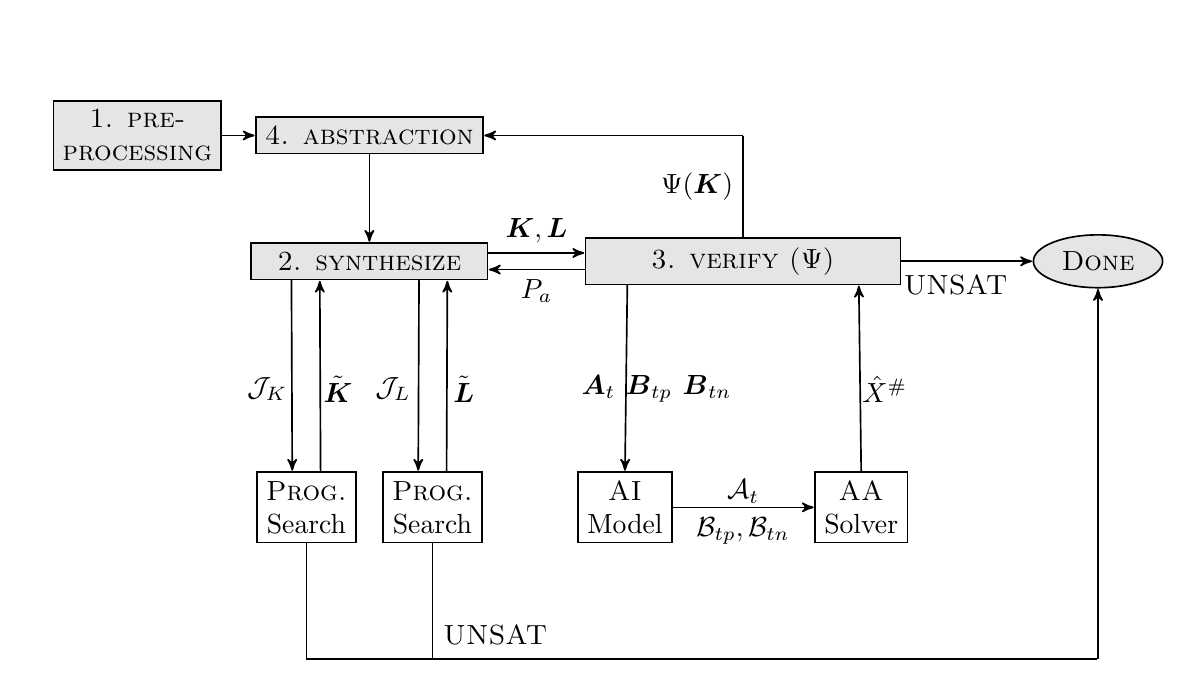
\begin{tikzpicture}[scale=0.3,->,>=stealth',shorten >=.2pt,auto, semithick, ampersand replacement=\&,]
  \matrix[nodes={draw, fill=none, shape=rectangle, minimum height=.2cm, minimum width=.2cm, align=center},row sep=.8cm, column sep=.2cm] {
   \coordinate (aux1);
   \& \coordinate (aux2);
   \& ;\\
   \&\node[fill=gray!20,align=center] (pre) {{\sc 1. pre-}\\{\sc processing}};
   \& \node[fill=gray!20,align=center] (abstract) {\sc 4. abstraction};
       % \node[draw=none] (FIK) at ([xshift=2.5cm,yshift=.3cm]abstract)  {\sc $\Psi (\mat{K})$};
   \& \coordinate (aux); \\ % \node[fill=yellow!20,align=center] (counter) {\sc counterexample};\\
   \& 
   \& \node[fill=gray!20,align=center, minimum width=3cm] (synth) {\sc 2. synthesize};
       %\node[draw=none] (KL) at ([xshift=2.5cm,yshift=-.25cm]synth)  {\sc $\mat{K},\mat{L}$};
       %\node[draw=none] (NKL) at ([xshift=2cm,yshift=1cm]synth)  {\sc $P_a$};
   \& \node[fill=gray!20,align=center, minimum width=4cm] (verify) {\sc 3. verify ($\Psi$)};
       %\node[draw=none] (VUNS) at ([xshift=.6cm,yshift=1cm]verify)  {\sc SAT};
       \node[draw=none] (SAT) at ([xshift=2.7cm,yshift=-.3cm]verify)  {\sc UNSAT};
   \& \node[ellipse, fill=gray!20] (done) {{\sc Done}};\\
   \&
   \& complexnode/.pic={
     \coordinate (auxsynth);
     \node[draw,rectangle,align=center] (KSAT) at ([xshift=-.8cm]auxsynth.center) {\sc Prog.\\Search};
     \node[draw,rectangle,align=center] (LSAT) at ([xshift=.8cm]auxsynth.center) {\sc Prog.\\Search};
     \node[draw=none] (SATK) at ([xshift=-.5cm,yshift=1.5cm]KSAT)  {$\mathcal{J}_K$};
     \node[draw=none] (K) at ([xshift=.4cm,yshift=1.5cm]KSAT)  {$\tilde{\mat{K}}$};
     \node[draw=none] (SATL) at ([xshift=-.5cm,yshift=1.5cm]LSAT)  {$\mathcal{J}_L$};
     \node[draw=none] (L) at ([xshift=.4cm,yshift=1.5cm]LSAT)  {$\tilde{\mat{L}}$};
    }
   \& complexnode/.pic={
     \coordinate (AA);
     \node[draw,rectangle,align=center] (AAI) at ([xshift=-1.5cm]AA.center) {\sc AI\\Model};
     \node[draw,rectangle,align=center] (AAV) at ([xshift=1.5cm]AA.center) {\sc AA\\Solver};
     \node[draw=none] (AB) at ([xshift=.4cm,yshift=1.5cm]AAI.center)  {\sc $\mat{A}_t$ $\mat{B}_{tp}$ $\mat{B}_{tn}$};     
     \node[draw=none] (MA) at ([yshift=.2cm]AA.center)  {$\mathcal{A}_t$};     
     \node[draw=none] (MB) at ([yshift=-.3cm]AA.center)  {$\mathcal{B}_{tp},\mathcal{B}_{tn}$}; 
     \node[draw=none] (AB) at ([xshift=0.3cm,yshift=1.5cm]AAV.center)  {\sl $\hat{X}^\#$};  
    }\\
   \&
   \& complexnode/.pic={
     \coordinate (UNSAT);
     \coordinate (KUNSAT)  at ([xshift=-.8cm]UNSAT.center);
     \coordinate (LUNSAT) at ([xshift=.8cm]UNSAT.center);
     \node[draw=none] (UNSATB) at ([xshift=1.6cm,yshift=.3cm]UNSAT)  {\sc UNSAT};
  }
  \& \& \coordinate (FAIL);\\
  };
  \path
    (pre.east) edge (abstract.west)
    (abstract.south) edge (synth.north)
    %([yshift=2em]synth.east) edge node {Candidate} ([yshift=2em]verif.west)
    %([yshift=-2em]verif.west) edge node {New input} ([yshift=-2em]synth.east)
    %([yshift=2em]synth.east) edge node[xshift=-0.7em] {Candidate} ([yshift=2em]verif.west)
    %([yshift=-2em]verif.west) edge node[xshift=-0.7em] {New input} ([yshift=-2em]synth.east)
    ([yshift=1em]synth.east) edge node {$\mat{K},\mat{L}$} ([yshift=1em]verify.west)
    ([yshift=-1em]verify.west) edge node {$P_a$} ([yshift=-1em]synth.east)
    (aux) edge (abstract.east) 
    (verify.east) edge (done.west);
  \path
    ([xshift=+.6cm]KSAT.north) edge ([xshift=-2.1cm]synth.south) 
    ([xshift=-3.3cm]synth.south) edge ([xshift=-.6cm]KSAT.north)
    ([xshift=.6cm]LSAT.north) edge ([xshift=3.3cm]synth.south)
    ([xshift=+2.1cm]synth.south) edge ([xshift=-.6cm]LSAT.north)
    ([xshift=-4.9cm]verify.south) edge (AAI.north)
    (AAI.east) edge (AAV.west)
    (AAV.north) edge ([xshift=4.9cm]verify.south)
    %(verify.north) edge (counter.south)
    %(counter.west) edge (abstract.east)
    %(counter.south west) edge (synth.north east)
    (FAIL.north) edge (done.south);
   \path[-] 
     (KSAT.south) edge (KUNSAT.north)
     (LSAT.south) edge (LUNSAT.north)
     (KUNSAT.east) edge (LUNSAT.west)
     (verify.north) edge node {$\Psi (\mat{K})$} (aux)
     (LUNSAT.east) edge (FAIL.west);
\end{tikzpicture}
}
\caption{CEGIS with abstraction refinement\label{fig:CEGARIS}.}
\end{figure}

%+++++++++++++++++++++++++++++++++++++++++++++++++++++++++++++++++++++++++++++++
\subsection{CEGIS with multi-staged verification}
\label{sec:CEGIS-precision-incrementation}
%+++++++++++++++++++++++++++++++++++++++++++++++++++++++++++++++++++++++++++++++

\begin{figure}[htb]
{\scriptsize
\centering
%\resizebox{.8\textwidth}{!}
{
 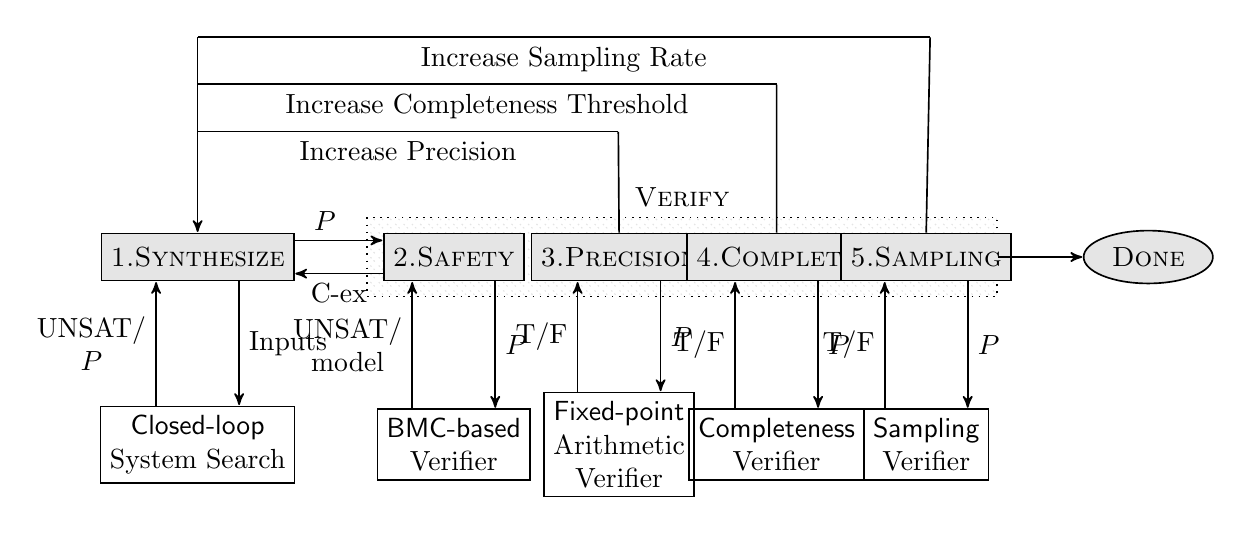
\begin{tikzpicture}[scale=0.3,->,>=stealth',shorten >=.2pt,auto, semithick, initial text=, ampersand replacement=\&,]
  \matrix[nodes={draw, fill=none, shape=rectangle, minimum height=.2cm, minimum width=.2cm, align=center
},
          row sep=.6cm, column sep=.9cm] {
   \coordinate (aux1);
   \& \coordinate (aux2);
   \&;\\
   \coordinate (aux3);
   \& \coordinate (aux4);
   \&;\\
   \coordinate (aux5);
   \& \coordinate (aux6);
   \&;\\
   \node[minimum width=1.5cm, minimum height=0.6cm, fill=gray!20] (synth) {{\sc 1.Synthesize}};
   \&
   complexnode/.pic={ 
     \node[rectangle,draw,dotted,
	minimum width=8cm,
	minimum height=1cm,
        pattern=north west lines, pattern color=gray!20,
	label={\sc Verify},] (verif) {};
     \node[minimum width=1cm, minimum height=0.6cm, fill=gray!20] (verif1) at ([xshift=-2.9cm]verif.center) {{\sc 2.Safety}};
     \node[minimum width=1cm, minimum height=0.6cm, fill=gray!20] (verif2) at ([xshift=-0.8cm]verif.center) {{\sc 3.Precision}};
     \node[minimum width=1cm, minimum height=0.6cm, fill=gray!20] (verif3) at ([xshift=1.2cm]verif.center) {{\sc 4.Complete}};
     \node[minimum width=1cm, minimum height=0.6cm, fill=gray!20] (verif4) at ([xshift=3.1cm]verif.center) {{\sc 5.Sampling}};
   } 
   \& \node[ellipse, fill=gray!20] (done) {{\sc Done}};\\
   \& \\
   \node[minimum height=0cm] (gp) {\sf Closed-loop \\ System Search};
   \&
   complexnode/.pic={ 
     \coordinate (aux);
   \node (bmc) at ([xshift=-2.9cm]aux.center) {\sf BMC-based \\Verifier};
   \node (fp)  at ([xshift=-.8cm]aux.center) {\sf Fixed-point \\ Arithmetic\\Verifier};
   \node (sv)  at ([xshift=1.2cm]aux.center) {\sf Completeness\\Verifier};
   \node (cv)  at ([xshift=3.1cm]aux.center) {\sf Sampling\\Verifier};
   }   
    \\
  };

   \path
    ([yshift=2em]synth.east) edge node[xshift=-0.5em,align=center] {$P$} ([yshift=2em]verif1.west)
    ([yshift=-2em]verif1.west) edge node {C-ex} ([yshift=-2em]synth.east)
    ([xshift=-5em]fp.north) edge node[align=center]  {T/F} ([xshift=-5em]verif2.south)
    ([xshift=-5em]sv.north) edge node[align=center]  {T/F} ([xshift=-5em]verif3.south)
    ([xshift=-5em]cv.north) edge node[align=center]  {T/F} ([xshift=-5em]verif4.south)
    ([xshift=5em]verif1.south) edge node[align=center] {$P$} ([xshift=5em]bmc.north)
    ([xshift=5em]verif2.south) edge node[align=center] {$P$} ([xshift=5em]fp.north)
    ([xshift=5em]verif3.south) edge node[align=center] {$P$} ([xshift=5em]sv.north)
    ([xshift=5em]verif4.south) edge node[align=center] {$P$} ([xshift=5em]cv.north)
    ([xshift=-5em]bmc.north) edge node[align=center]  {UNSAT/\\model} ([xshift=-5em]verif1.south)
    (verif) edge node {} (done)
    ([xshift=5em]synth.south) edge node[align=center] {Inputs} ([xshift=5em]gp.north)
    ([xshift=-5em]gp.north) edge node[align=center] {UNSAT/\\$P$} ([xshift=-5em]synth.south)
    (aux1) edge (synth.north);
   \path[-]
   (verif2.north) edge node[align=center] {} ([xshift=-2.7cm]aux6)
   ([xshift=-2.7cm]aux6) edge node[align=center] {Increase Precision} (aux5)
   (verif3.north) edge node[align=center] {} ([xshift=4cm]aux4)
   ([xshift=4cm]aux4) edge node[align=center] {Increase Completeness Threshold} (aux3)
   (verif4.north) edge node[align=center] {} ([xshift=10.5cm]aux2)
   ([xshift=10.5cm]aux2) edge node[align=center] {Increase Sampling Rate} (aux1);

 \end{tikzpicture}
}}
\caption{CEGIS with multi-staged verification.}
\label{fig:CEGIS-precision-increment}
\end{figure}

%\subsubsection{Controller synthesis}

The controller synthesis is described in Fig.~\ref{fig:CEGIS-precision-increment}.
One important observation is that, for this approach,
we compute the set of reachable states by finding 
a completeness threshold $\overline{k}$.
Essentially, $\overline{k}$ represents the number of iterations 
required to sufficiently unwind the closed-loop state-space system 
such that the boundaries are not violated for any $k>\overline{k}$
(i.e. it's sufficient to unwound the closed-loop state-space system up to  
$\overline{k}$ in order to ensure that $\phi_{safety}$ holds). 

Next, we describe the different phases in Fig.~\ref{fig:CEGIS-precision-increment}
(blocks 1 to 5):

1. The inductive synthesis phase (i.e. {\sc synthesize}) uses BMC to
compute a candidate solution $K$. It does this by assuming some 
precision $<I_p,F_p>$ for the plant, a $k$ and a sampling rate.  The checks that
these assumptions are sound are performed by the subsequent {\sc
  verify} stages.

2. The first {\sc verify} stage, {\sc safety}, 
performs potentially unsound operations by considering the currently
assumed $<I_p,F_p>$, $k$ and sampling rate. % The soundness is to be 
% restored by the subsequent three validation stages.

3. The second {\sc verify} stage, {\sc precision}, 
 restores soundness with respect to the plant's precision
by using interval arithmetic \cite{moore1966interval} to validate the 
operations performed by the previous stage.

4. The third {\sc verify} stage, {\sc complete}, checks that the
current $k$ is large enough to ensure that the boundaries are not
violated for any $k'>k$.  For this purpose, we compute the
completeness threshold $\overline{k}$ for the current candidate $K$
and check that $k{\leq}\overline{k}$.  \todo{discuss the computation
  of the completeness threshold}

5. The last {\sc verify} stage, {\sc sampling}, 
ensures that the current sampling rate is large enough by using an 
external checker (\todo{add more details here once we have them}).


%-------------------------------
\section{Experimental Evaluation}
%-------------------------------


%-------------------------------
\subsection{Description of the benchmarks}
%-------------------------------

A set of state-space models for different classes of 
systems were extracted from the literature and employed 
for validating our automated synthesis methodology. 
All the systems are SISO models of the following form:
%
\begin{equation}
\left\lbrace\begin{array}{c}
\dot{\textbf{x}}(t)=\textbf{A}\textbf{x}(t)+\textbf{B}u(t)\\
y(t)=\textbf{C}\textbf{x}(t)+\textbf{D}u(t)
\end{array}\right.
\end{equation}

Table~\ref{table:State-space benchmarks} summarizes all benchmarks extracted 
from the control system literature~\cite{Franklin15,maglev,converters,CTMS}. 
\textit{DC Motor Position and Rate} plants describes the angular position and 
velocity of a DC Motor, respectively, that coupled with wheels and cables provides 
translational motion. 
\textit{Aircraft Pitch Dynamics} plant represents the air vehicle orientation and 
control based on the pitch dimension. 
\textit{Ball Magnetic Levitation} plant describes a physical model to keep a 
metal ball hanged in air via a magnetic field . 
\textit{Buck Converter} plant represents a power converter model that steps down 
voltage from the supply to the load while stepping up current. 
\textit{Boost Converter} plant also represents a power converter model, but here 
it steps up voltage from the supply to the load while stepping down current. 
\textit{Buck-boost Converter} plant represents a converter model that has an output 
voltage magnitude, which is either greater than or less than the input voltage magnitude. 

\textit{Automotive Cruise System} plant describes a physical model that represents 
the speed of a motor vehicle. 
\textit{Helicopter Longitudinal Motion} plant provides the 
longitudinal motion model of a helicopter. 
\textit{Inverted Pendulum} plant describes a pendulum model
with its center of mass above its pivot point. 
\textit{Magnetic Suspension} plant provides the physical model for which 
a given object is suspended via a magnetic field. 
\textit{Magnetized Pointer} plant describes a physical model that is rotated through interaction 
with magnetic fields (typically employed in analog gauges and indicators).
\textit{1/4 Car Suspension} plant presents a physical model that connects a car to its wheels 
and allows relative motion between both parts.
\textit{Computer Tape Driver} plant describes a physical model to read and write data 
on a storage device in the computer.
\textit{USCG Cutter Tampa Heading Angle} plant presents a physical model 
for the yaw angle dynamics of a US warship USCG Cutter Tampa.

All benchmarks were discretized with different sample times using 
the approach described in the Appendix~\ref{sec:appendix}. 
All experiments were performed considering $x_{i}^{-}=-1$ and 
$x_{i}^{+}=1$ and the inputs $u_{k}=0, \forall k>0$.

We have also conducted the experimental evaluation on a 12-core 2.40 GHz
Intel Xeon E5-2440 with 96 GB of RAM and Linux OS. All times given are wall 
clock time in seconds as measured by the UNIX date command. 

\textcolor{red}{we have to describe the timeout...}

%
\begin{table}[htb]
\centering
\footnotesize
\caption{Benchmarks for State-Space Physical Plants.}
\label{table:State-space benchmarks}
\begin{tabular}{|c|c|c|c|c|}
\hline
%\textbf{ID \#} & 
\textbf{System}                                                               & \textbf{A} & \textbf{B} & \textbf{C} & \textbf{D} \\ \hline
%1              & 
\begin{tabular}[c]{@{}c@{}}DC Motor\\ Position\end{tabular}                   & $\left[\begin{array}{ccc}
0		& 1 		& 0						\\
0 		& -1.087	& 8587					\\
0		& -9964		& -1.455\times 10^{6}	\\
\end{array}\right]$ & $\left[\begin{array}{c}
0 \\ 0 \\ -1.455\times10^{6}
\end{array}\right]$           & $\left[\begin{array}{ccc}
1 & 0 & 0\\
\end{array}\right]$ & 0 \\  \hline
%2              & 
\begin{tabular}[c]{@{}c@{}}Aircraft \\ Pitch\\ Dynamics\end{tabular} & $\left[\begin{array}{ccc}
-0.313	& 56.7 		& 0		\\
-0.0139	& -0.426	& 0		\\
0		& 56.7		& 0		\\
\end{array}\right]$ & $\left[\begin{array}{c}
0.232 \\ 0.0203 \\ 0
\end{array}\right]$ & $\left[\begin{array}{ccc}
1 & 0 & 0\\
\end{array}\right]$ & 0 \\ \hline
%3            & 
\begin{tabular}[c]{@{}c@{}}Ball\\ Magnetic\\ Levitation\end{tabular} & $\left[\begin{array}{ccc}
0		& 1 		& 0		\\
1752	& 0			& -34.07\\
0		& 0			& -38.27\\
\end{array}\right]$ & $\left[\begin{array}{c}
0 \\ 0 \\ 1.923
\end{array}\right]$ & $\left[\begin{array}{ccc}
1 & 0 & 0\\
\end{array}\right]$ & 0 \\ \hline
%4              & 
\begin{tabular}[c]{@{}c@{}}Buck\\ Converter\end{tabular}                      & $\left[\begin{array}{cc}
0		& -500 \\
4545	& -1515\\
\end{array}\right]$ & $\left[\begin{array}{c}
125 \\ 0 \\
\end{array}\right]$ & $\left[\begin{array}{cc}
 0 & 1\\
\end{array}\right]$ & 0 \\ \hline
%5              & 
\begin{tabular}[c]{@{}c@{}}Boost\\ Converter\end{tabular} & $\left[\begin{array}{cc}
0		& -375 \\
3409	& -1515\\
\end{array}\right]$ & $\left[\begin{array}{c}
500 \\ 0 \\
\end{array}\right]$ &  $\left[\begin{array}{cc}
0 & 1\\
\end{array}\right]$  & 0        \\ \hline
%6              & 
\begin{tabular}[c]{@{}c@{}}Buck-boost\\ Converter\end{tabular} & $\left[\begin{array}{cc}
0		& 375 \\
-3409	& -1515\\
\end{array}\right]$ & $\left[\begin{array}{c}
125 \\ 0 \\
\end{array}\right]$ & $\left[\begin{array}{cc}
0 & 1\\
\end{array}\right]$ & 0 \\ \hline
%7              & 
\begin{tabular}[c]{@{}c@{}}Automotive\\ Cruise\\ System\end{tabular} & -0.05 & 0.03125 & 0.032 & 0 \\ \hline
%8              & 
\begin{tabular}[c]{@{}c@{}}DC Motor\\ Rate\end{tabular} & $\left[\begin{array}{cc}
-1000		& -13 \\
-8			& 0\\
\end{array}\right]$ & $\left[\begin{array}{c}
4 \\ 0 \\
\end{array}\right]$ & $\left[\begin{array}{cc}
0 & 6.25\\
\end{array}\right]$ & 0 \\ \hline
%9              & 
\begin{tabular}[c]{@{}c@{}}Helicopter\\ Longitudinal\\ Motion\end{tabular}    & $\left[\begin{array}{ccc}
-0.42		& 0.0168		& -0.396	\\
0.5			& 0				& 0			\\
0			& 0.5 			& 0			
\end{array}\right]$ & $\left[\begin{array}{c}
16 \\ 0 \\ 0
\end{array}\right]$ & $~
\left[\begin{array}{ccc}
0.6125	& -0.6125	& 15.44 \\
\end{array}\right]$ & 0 \\ \hline
%10             & 
Pendulum   & $\left[\begin{array}{cc}
0		& -2.453	\\
4		& 0			\\	
\end{array}\right]$ & $\left[\begin{array}{c}
4 \\ 0
\end{array}\right]$ & $\left[\begin{array}{cc}
-1.225	& -2.15 	\\
\end{array}\right]$           & 9.8           \\ \hline
%11             & 
\begin{tabular}[c]{@{}c@{}}Inverted\\ Pendulum\end{tabular} & $\left[\begin{array}{cccc}
0		& 1		& 0 	& 0	\\
1		& 0		& 0		& 0	\\
0		& 1 	& 0		& 0 \\
0		& 0		& 1 	& 0 \\	
\end{array}\right]$ & $\left[\begin{array}{c}
1 \\ 0 \\ 0 \\ 0
\end{array}\right]$  & $\left[\begin{array}{cccc}
0	& 0	& 1 & -0.75 \\
0	& 1	& 0	& 0		
\end{array}\right]$ & $\left[\begin{array}{c}
0 \\
0 \end{array}\right]$ \\ \hline
%12             & 
\begin{tabular}[c]{@{}c@{}}Magnetic\\ Suspension\end{tabular} & $\left[\begin{array}{cc}
0		& 31.25	\\
32		& 0		\\	
\end{array}\right]$ & $\left[\begin{array}{c}
8 \\ 0
\end{array}\right]$ & $\left[\begin{array}{cc}
0	& 9.766 	\\
\end{array}\right]$ & 0 \\ \hline
%13             & 
\begin{tabular}[c]{@{}c@{}}Magnetic\\ Pointer \end{tabular} & $\left[\begin{array}{ccc}
-0.271		& -0.05336	& 0	\\
0.03125		& 0			& 0	\\
0			& 0.01562 	& 0	\\	
\end{array}\right]$ & $\left[\begin{array}{c}
1 \\ 0 \\ 0
\end{array}\right]$ & $\left[\begin{array}{ccc}
0	& -0.5888	& -0.2562 \\
\end{array}\right]$ & 0           \\ \hline
%14             & 
\begin{tabular}[c]{@{}c@{}}1/4 Car\\ Suspension\end{tabular} & $
\left[\begin{array}{cccc}
-516.1	& -222.1& -79.75& -33.06	\\
256		& 0		& 0		& 0			\\
0		& 64 	& 0		& 0 \\
0		& 0		& 32 	& 0 \\	
\end{array}\right]$ & $\left[\begin{array}{c}
8 \\ 0 \\ 0 \\ 0
\end{array}\right]$ & $\left[\begin{array}{cccc}
0	& 0	& 9.969 & 4.133 \\
\end{array}\right]$ & 0 \\ \hline
%15             & 
\begin{tabular}[c]{@{}c@{}}Computer\\ Tape\\ Driver\end{tabular} & $\left[\begin{array}{ccc}
-1760		& -976.6	& -457.8	\\
1024		& 0			& 0			\\
0			& 512 		& 0			\\	
\end{array}\right]$ & $\left[\begin{array}{c}
8 \\ 0 \\ 0
\end{array}\right]$ & $\left[\begin{array}{ccc}
1.5	& 2.051	& 1.144 \\
\end{array}\right]$ & 0           \\ \hline
%16             & 
\begin{tabular}[c]{@{}c@{}}USCG \\ Cutter\\ Tampa\\ Heading\\ Angle\end{tabular} & $\left[\begin{array}{ccc}
-0.271		& -0.05336	& 0	\\
0.03125		& 0			& 0			\\
0			& 0.01562 	& 0			\\	
\end{array}\right]$ & , $\left[\begin{array}{c}
1 \\ 0 \\ 0
\end{array}\right]$ & $\left[\begin{array}{ccc}
0	& -0.5888	& -0.2562 \\
\end{array}\right]$ & 0 \\ \hline
\end{tabular}
\end{table}


%-------------------------------
\subsection{Objectives}
%-------------------------------

%-------------------------------
\subsection{Results}
%-------------------------------


%-------------------------------
\subsection{Threats to validity}
%-------------------------------


%% %-------------------------------
%% \section{Related Work}
%% \label{sec:rw}
%% %-------------------------------


%-------------------------------
\section{Extensions}
\label{sec:extensions}
%-------------------------------

%-------------------------------
\subsection{LTI systems with output} 
\label{ssec:LTI}
%-------------------------------

LTI models in the form: 
%
\begin{align}
\label{eq:ode}
\dot{\vec{x}}(t)&=\mat{A}\vec{x}(t)+\mat{B}\vec{u}(t)\ \ :\ \ \vec{x} \in \mathbb{R}^{n}, \vec{u} \in \mathbb{R}^m, \mat{A} \in \mathbb{R}^{n \times n},\mat{B} \in \mathbb{R}^{n \times m}\\
\vec{y}(t)&=\mat{C}\vec{x}(t)+\mat{D}\vec{u}(t)\ \ :\ \ \vec{y} \in \mathbb{R}^{o}, \mat{C} \in \mathbb{R}^{o \times n}, \mat{D}  \in \mathbb{R}^{o \times m}\nonumber
\end{align}
\noindent where $\dot{\vec{x}}(t)$ describes the state evolution equation; 
$\vec{y}(t)$ represents an instantaneous output equation; and $\mat{A}$, $\mat{B}$, $\mat{C}$, and $\mat{D}$ are matrices that fully specify 
a continuous plant. Eq.~\eqref{eq:ode} is soundly discretized 
(as shown in the appendix) into
%
\begin{align}
\label{eq:plant}
\vec{x}_{k+1}&=\mat{A}_d\vec{x}_k+\mat{B}_d\vec{u}_k\\
\vec{y}_k&=\mat{C}_d\vec{x}_k+\mat{D}_d\vec{u}_k .\nonumber
\end{align}
%


\newpage

\bibliographystyle{abbrv}
\bibliography{paper}  
%\begin{thebibliography}{4}
%\end{thebibliography}

\newpage
\appendix
%-------------------------------
\section{Stability of closed-loop systems}
\label{sec:appendix-stability}
%-------------------------------

%\todo{[Here discuss Jury criterium for DISCRETE-TIME models - a simplified version of the first part of what is now in Section \ref{sec:cof_verification} (with no quantisation noises yet).]}  

A discrete-time system is asymptotically stable if and only if all the roots 
of the characteristic polynomial ({\it i.e.}, the eigenvalues) are inside of 
the unity circle, {\it i.e.}, their absolute value are less than 
one~\cite{astrom1997computer}. In this paper, we express 
the stability specification $\phi_{stability}$ in terms of  
Jury's criterion \cite{fadali}. A detailed description of this 
specification can be found in the Appendix~\ref{sec:appendix-stability}.

For a closed-loop system as~\eqref{eq:closedloopss}, 
the characteristic polynomial $P(z)$ should be computed as follows:
\begin{equation}
P(z)= \det( z I_{n} - A_d + B_d K ),
\end{equation}
where $I_{n}$ is the n-th order identity matrix. 

Jury's criterion provides necessary and sufficient conditions for the eigenvalues 
to be within the unit circle and, consequently, the system is stable.  Given a 
polynomial $P(z)$ of the form
$$
P(z) = a_{0}z^{N} + a_{1}z^{N-1} + ... a_{N-1}z + a_{N} = 0, a_{0}\neq 0,
$$
Jury's criterion explores solely the coefficients ($a_{0},a_{1},...,a_{N-1}$) 
of $P(z)$ for checking the validity of the stability property $\phi_{stability}$. 

In particular, Jury stability test is already explained in the control system 
literature ({\it e.g.}~\cite{fadali}). This study, however, limits itself to 
explain the encoding of Jury's criterion for the formal synthesis purpose. 
For the stability  test procedure, the following Jury matrix 
$M=[m_{ij}]_{(2N-2)\times N}$ is built  from $P(z)$ coefficients:
$$
M=\left[
\begin{matrix}
  V^{(0)} \\
  V^{(1)} \\
  \vdots \\
  V^{(N-2)}
 \end{matrix}
\right]\mbox{,}
$$
\noindent where $V^{(k)}=[v^{(k)}_{ij}]_{2\times N}$ such that
$$
v^{(0)}_{ij}=\begin{cases} 
a_{j-1}, & \mbox{if } i=1 \\   v^{(0)}_{(1)(N-j+1)}, & \mbox{if } i=2 
\end{cases}\mbox{, and} 
$$
$$
v^{(k)}_{ij}=\begin{cases} 
0, & \mbox{if } j>n-k\\
v^{(k-1)}_{1j}-v^{(k-1)}_{2j}\cdot\frac{v^{(k-1)}_{11}}{v^{(k-1)}_{21}}, & \mbox{if } j\leq n-k  \mbox{ and } i=1 \\
v^{(k)}_{(1)(N-j+1)}, & \mbox{if } j\leq n-k \mbox{ and } i=2 \\
\end{cases} \mbox{,}
$$
\noindent where $k\in\mathbb{Z}$, such that $0<k<N-2$. $P(z)$ is the 
characteristic polynomial of a stable system if and only if the following 
four propositions hold:
\begin{itemize}
\item $R_{1}$: $S(1)>0$;
\item $R_{2}$: $(-1)^{N}P(-1)>0$;
\item $R_{3}$: $\vert{a_{0}}\vert <a_{N}$;
\item $R_{4}$: $m_{11}>0\iff m_{31}\wedge m_{51}\wedge \dots \wedge m_{(2N-3)(1)}$.
\end{itemize}

The stability property $\phi_{stability}$ is then encoded as follows:
$$
\phi_{stability}\iff \ (R_{1} \wedge R_{2} \wedge R_{3} \wedge R_{4}).
$$


%+++++++++++++++++++++++++++++++++++++++++++++++++++++++++++++++++++++++++++++++
\section{LTI system Transformations and Equivalencies} \label{sec:appendix}
%+++++++++++++++++++++++++++++++++++++++++++++++++++++++++++++++++++++++++++++++

%+++++++++++++++++++++++++++++++++++++++++++++++++++++++++++++++++++++++++++++++
\subsection{Discretising continuous space dynamics}
%+++++++++++++++++++++++++++++++++++++++++++++++++++++++++++++++++++++++++++++++

A dynamical system is a system in which a function describes the progression of a state over time. 
In a continuous domain with linear dynamics, it is described by a first order Ordinary Differential Equation (ODE).
\begin{equation}
\dot{x}(t)=\vec{A}\vec{x}(t)+\vec{B}\vec{u}(t) +\vec{w}(t).
\label{eq:dynamical}
\end{equation}

\noindent with $\vec{w} \sim \mathcal{N}(0,Q)$.\\
Furthermore, a control system may have a derived output that is a linear combination of its states and inputs, 
which may restrict the observability of the state-space from the output space.
\begin{equation}
\vec{y}(t)=\vec{C}\vec{x}(t)+\vec{D}\vec{u}(t).
\end{equation}

Discretization of an continuous dynamical system turns the ODE into a difference equation, assuming zero-order hold
for the input $\vec{u}$ and continuous integration for the noise $\vec{w}$, to
\begin{align}
\label{eq:discretization}
\vec{x}_{k+1} &= \vec{A}_d\vec{x}_k+\vec{B}_d\vec{u}_k + \vec{w}_k,\\
y_k &= \vec{C}_d \vec{x}_ k + \vec{D}_d \vec{u}_ k. 
\end{align}
with covariance for $\vec{w}_k \sim \mathcal{N}(0,Q_d)$,
where
\begin{align}
\label{eq:discretize}
\vec{A}_d &= e^{\vec{A} T_s} = \mathcal{L}^{-1} { ( s \vec{I} - \vec{A} )^{-1} }_{t = T_s},\\
\vec{B}_d &= \int_{0}^{T_s} e^{\vec{A} t} dt\ \vec{B} = \vec{A}^{-1} ( \vec{A}_d - \vec{I} ) \vec{B},\\
\vec{C}_d &= \vec{C},\\
\vec{D}_d &= \vec{D},\\
Q_d &= \int_{0}^{T_s} e^{\vec{A} t} Q e^{\vec{A}^T t} dt.
\end{align}
and $T_s$ is the sample time. Then
\begin{align*}
x(kT)=x_k \wedge y(kT) = y_k, \forall k.
\end{align*}
Let $g_d(k)=\mathcal{G}(t,g(t),T)$ be a function that performs the discretization described above, where $g(t)$
represents the continuous dynamics and $g_d(k)$ the corresponding discrete dynamics. 
Let $G(s)=\mathcal{L}(g(t))$ and $G_d(z)=\mathcal{Z}(g_d(k))$ be the corresponding Laplace and Z-transforms
of $g(t)$ and $g_d(k)$. Given this relation, we have 
$$G_d(z)=G(z)|_{z=e^{sT}} : g_d(k)=\mathcal{G}(t,g(t),T) \wedge T < \frac{1}{.5f_s},$$
where $.5f_s$ is the Nyquist frequency of $g(t)$. This last restriction is introduced to avoid the effects of aliasing
which could cause ``phantom poles'' to appear otherwise. 
The eigenvalues of $\vec{A}_d$ corresponding to the poles of $G_d(z)$, and those of $\vec{A}$ corresponding to the poles of $G(s)$ are similarly related.
$\hat{\lambda}_i=e^{-\lambda_iT} : \hat{\lambda}_i \in \sigma(\vec{A}_d) \wedge \lambda_i \in \sigma(\vec{A})$
where $\sigma(\cdot)$ is the spectrum of a matrix.
The following remark is worth mentioning regarding the above.
\begin{remark}
The witnessed maximum amplitude of the discrete signals $x_k,y_k$ may be smaller to that of $x(t),y(t)$ due to synchronism at fraction-frequency sampling.
This means that reasoning about the state-space must consider the effects of this possibility as well of the case of maximal inputs from the continuous specification.
\end{remark}
 Since \eqref{eq:discretization} is a bisimulation of \eqref{eq:ode}, we may use the semantics in section \ref{sec:model_semantics} to model continuous dynamical systems.

%+++++++++++++++++++++++++++++++++++++++++++++++++++++++++++++++++++++++++++++++
\subsection{Modelling quantization as noise}
%+++++++++++++++++++++++++++++++++++++++++++++++++++++++++++++++++++++++++++++++

During any given ADC conversion, the continuous signal will be sampled in the real domain and transformed into a $\mathbb{R}\langle I_{adc},F_{adc} \rangle$ value. this sampling uses a threshold which is defined by the less significant bit ($q_{adc}=2^{-F_{adc}}$) of the adc and some nonlinearities of the circuitry. The overall conversion is
$$\mathcal{F}\langle I_{adc},F_{adc} \rangle(y(t)) = y_k : y_k \in \left[y(t)-\frac{q_{adc}}{2}\ \ \ \ y(t)+\frac{q_{adc}}{2}\right]$$.
If we denote the error in the conversion as $\nu_k=y_k-y(t) : t=nk$ then we may define some bounds for it $\nu_k \in [-\frac{q_{adc}}{2}\ \ \frac{q_{adc}}{2}]$.

We will assume, for the purposes of this analysis, that the domain of the ADC is that of the digital controller (\emph{ie} the quantizer includes any digital gain added in the code).
The process of quantization in the DAC is similar except that it is going from $\mathbb{R}\langle I_{adc},F_{adc} \rangle \rightarrow \mathbb{R}\langle I_{dac},F_{dac} \rangle$. If these domains are the same ($I_{adc}=I_{dac},F_{adc}=F_{dac}$), or if the DAC resolution in higher than the ADCs, then the DAC quantization error is equal to zero.
From the above equations we can now infer that $\nu_1 \in [-\frac{q_1}{2}\ \ \frac{q_1}{2}], \nu_2 \in [-\frac{q_2}{2}\ \ \frac{q_2}{2}] : q_1=q_{adc} \wedge q_2=q_{dac}$.
Note that these bounds hold irrespective of whether the noise is correlated, hence we may use them to overapproximate the effect of the noise on the state space progression over time.
The resulting dynamics are:
\begin{align}
\label{eq:pre_quantization}
\vec{x}_{k+1} &= \vec{A}_d\vec{x}_k+\vec{B}_d(\vec{u}_k+{\vec{\nu}_2}_k) + \vec{w}_k,\\
y_k &= \vec{C}_d \vec{x}_ k + \vec{D}_d \vec{u}_ k+{\vec{\nu}_1}_k. 
\end{align}

Which, when modelled into closed loop dynamics results in:

\begin{align}
\label{eq:quantization}
\vec{x}_{k+1} &= (\vec{A}_d-\vec{B}_d\mat{K}_d\mat{C}_d) \vec{x}_k+\vec{B}_d{\vec{\nu}_2}_k + \vec{w}_k,\\
y_k &= \vec{C}_d \vec{x}_ k + \vec{D}_d \vec{u}_ k+{\vec{\nu}_1}_k. 
\end{align}

%+++++++++++++++++++++++++++++++++++++++++++++++++++++++++++++++++++++++++++++++
\subsection{Controllable canonical form} \label{sec:reachable}
%+++++++++++++++++++++++++++++++++++++++++++++++++++++++++++++++++++++++++++++++

Let us have a discrete time SISO system with an $n^{th},m^{th} : n\geq m$ order armax model
$$y[k]=\sum_{i=1}^n a_iy[k-i]+\sum_{i=0}^m b_iu[k-i],$$
where $y$ is the output of the system and $u$ its input.
The equivalent LTI dynamics of such a model are:
\begin{align}
\label{eq:cf_SISO}
\vec{x}_{k+1}=&\mat{A}_{cf}\vec{x}_k+\mat{B}_{cf}u_k : \vec{x}_k=[y_{k-n}\ \hdots y_{k-1}\ y_{k}]^T\\
y_k=&\mat{C}_{cf}\vec{x}_k + b_0u_k\nonumber\\
\mat{A}_{cf}=&\left[
\begin{array}{ccccc}
0&1&0&\cdots&0\\
0&0&1&\cdots&0\\
\vdots&\vdots&\vdots&\ddots&\vdots\\
0&0&0&\cdots&1\\
-a_n&-a_{n-1}&-a_{n-2}&\cdots&-a_1
\end{array}\right],
\mat{B}_{cf}=\left[
\begin{array}{c}
0\\0\\ \vdots\\ 0\\ 1
\end{array}\right]\nonumber\\
\mat{C}_{cf}=&[\begin{array}{ccccc}b_n-a_nb_0&b_{n-1}-a_{n-1}b_0&\cdots&b_1-a_1b_0\end{array}] : b_{i \in (m\ n]}=0\nonumber
\end{align}

where the coefficients $a_i$ describe the characteristic polynomial of the system. This matrix shape is
called a Controllable Canonical Form because the dynamics of the feedback are directly related to these
coefficients. Specifically, given a feedback controller $\mat{K}$ for this system, the closed loop dynamics
will have the shape
\begin{align}
\mat{A}_{cf}+\mat{B}_{cf}\mat{K}_{cf}=&\left[
\begin{array}{ccccc}
0&1&0&\cdots&0\\
0&0&1&\cdots&0\\
\vdots&\vdots&\vdots&\ddots&\vdots\\
0&0&0&\cdots&1\\
k_n-a_n&k_{n-1}-a_{n-1}&k_{n-2}-a_{n-2}&\cdots&k_1-a_1
\end{array}\right]
\label{eq:cf_SISO_fb}
\end{align}
which means we can directly modify each coefficient by selecting a controller parameter.
In the MIMO case, the Controllable Canonical Form has the following shape:
\begin{align}
\mat{A}_{cf}=&\left[
\begin{array}{ccccc}
0&\mat{I}_{n-1}&0&\cdots&0\\
0&0&\mat{I}_{n-2}&\cdots&0\\
\vdots&\vdots&\vdots&\ddots&\vdots\\
0&0&0&\cdots&1\\
-\mat{a_n}\mat{M}_n&-\mat{a_{n-1}}\mat{M}_{n-1}&-\mat{a_{n-2}}\mat{M}_{n-2}&\cdots&-\mat{a_1}\mat{M}_{1}
\end{array}\right],
\mat{B}_{cf}=\left[
\begin{array}{c}
0\\0\\ \vdots\\ 0\\ \mat{M}_0
\end{array}\right]\nonumber\\
\mat{C}_{cf}=&[\begin{array}{ccccc}\mat{\eta}_n&\mat{\eta}_{n-1}&\cdots&\mat{\eta}_1\end{array}] :
\mat{I}_i,\mat{M}_i \in \mathbb{R}^{q_i \times q_i} \wedge \mat{a}_i \in \mathbb{R}^{q \times q_i} \wedge \mat{\eta}_i \in \mathbb{R}^o \wedge  \mat{\eta}_{i \in (m\ n]}=0 \nonumber
\label{eq:cf_MIMO}
\end{align}
where $q$ is the number of inputs, $q_i$ the number of inputs with a transfer function of order of at least $i$, $\mat{I}_i$ an identity matrix, $\mat{M}_i$ an upper triangular matrix with 1s in its diagonal, $\mat{a_i}$ a matrix of coefficients of the $i^th$ order on its diagonal, and $o$ the number of outputs. Ideally we aim for $\mat{M}_i=\mat{I}_i, \forall i>0$

Any LTI system can be transformed into a controllable canonical form by a matrix $\mat{T} : \vec{x}=\mat{T}\hat{\vec{x}}$
Then the dynamics of the controllable form are
\begin{align}
\hat{\vec{x}}_{k+1}=&\mat{A}_{cf}\hat{\vec{x}}_k+\mat{B}_{cf}u_k : \mat{A}_{cf}=\mat{T}\mat{A}\mat{T}^{-1} \wedge \mat{B}_{cf}=\mat{T}\mat{B}\\
y_k=&\mat{C}_{cf}\hat{\vec{x}}_k + b_0u_k : \mat{C}_{cf}=\mat{C}\mat{T}^{-1}\nonumber
\end{align}
where $\mat{T}$ can be calculated as follows:

Let 
\begin{equation}
\mat{R}=[\begin{array}{ccccc}\mat{B}&\mat{A}\mat{B}&\mat{A}^2\mat{B}&\hdots&\mat{A}^{n-1}\mat{B}\end{array}]
\label{eq:rncf}
\end{equation}
be the reachability matrix of the system, and
\begin{equation}
\mat{R}_{cf}=\left[\begin{array}{ccccc}1&a_1&a_2&\hdots&a_{n-1}\\0&1&a_1&\hdots&a_{n-2}\\ \vdots&\ddots&\ddots&\ddots&\ddots\end{array}\right]
\label{eq:rcf}
\end{equation}
the reachability matrix of the canonical form. Then 
\begin{equation}
\mat{T}=\mat{R}_{cf}\mat{R}^{-1}
\label{eq:to_cf}
\end{equation}

%+++++++++++++++++++++++++++++++++++++++++++++++++++++++++++++++++++++++++++++++
\subsection{Observable canonical form} \label{sec:observable}
%+++++++++++++++++++++++++++++++++++++++++++++++++++++++++++++++++++++++++++++++
The Controllable Canonical Form is ideal when we have access to the state space. However, in most cyberphisical
systems, only the outputs of the plant can be observed, hence we require an Observable Canonical Form.
For SISO systems, this is:
\begin{align}
\label{of_SISO}
\mat{A}_{of}=&\left[
\begin{array}{ccccc}
0&0&0&\cdots&-a_n\\
1&0&0&\cdots&-a_{n-1}\\
0&1&0&\cdots&-a_{n-2}\\
\vdots&\ddots&\ddots&\ddots&\vdots\\
0&0&\cdots&1&-a_1
\end{array}\right],
\mat{B}_{of}=\left[
\begin{array}{c}
\eta_n\\ \eta_{n-1}\\ \vdots\\ \eta_1
\end{array}\right]\\
\mat{C}_{of}=&[\begin{array}{ccccc}0&0&\cdots&0&1\end{array}] \nonumber
\end{align}

What is important to notice her is that $\mat{A}_{of}=\mat{A}_{cf}^T, \mat{C}_{of}=\mat{B}_{cf}^T$
and $\mat{B}_{of}=\mat{C}_{cf}^T$, which also applies to the MIMO case.

Let 
\begin{equation}
\label{eq:wnof}
\mat{W}_o=[\begin{array}{ccccc}\mat{C}&\mat{A}\mat{C}&\mat{A}^2\mat{C}&\hdots&\mat{C}^{n-1}\mat{B}\end{array}]^T
\end{equation}
be the observability matrix of the system, and
\begin{equation}
\label{eq:wof}
\mat{W}_{of}=\mat{R}_{cf}^{-1}
\end{equation}
the observability matrix of the canonical form (see eg~\cite{astrom1997computer}). 
Then the dynamical system 
\begin{equation}
\label{eq:to_of}
\hat{\vec{x}}_{k+1}=(\mat{A}_o-\mat{L}\mat{C}_o)\hat{\vec{x}}_k+\mat{B}_o\vec{u}+\mat{L}\vec{y} : \mat{L}=\mat{W}_o^{-1}\mat{W}_{of} \left[ \begin{array}{c}p_1-a_1\\p_2-a_2\\p_n-a_n\end{array}\right]
\end{equation}
\begin{displaymath}
\mat{A}_o=\mat{A},\ \mat{B}_o=\mat{B},\ \mat{C}_o=\mat{C}
\end{displaymath}
is an observer of the system $\vec{x}_{k+1}=\mat{A}\vec{x}+\mat{B}\vec{u} : \vec{y}=\mat{C}\vec{x}$. $p_i$ are user selected
values which will affect the error of the observer estimator. The differentiation between $\mat{*}_o$ and $\mat{*}$ will be exploited later in this work. For the time being we will assume they are the same.

Figure \ref{fig:observersystem} shows an LTI system with a feedback control using an observer. Presuming a sampled model of the plant as described in \eqref{eq:discretize}, the closed loop dynamics of this system are given by:
\begin{equation}
\left [\begin{array}{c}\vec{x}\\ \hat{\vec{x}}_e \end{array}\right]_{k+1}
=\left [\begin{array}{cc}\mat{A}_d-\mat{B}_d\mat{K}_d&\mat{B}_d\mat{K}_d\\ \mat{0}&\mat{A}_d-\mat{L}_d\mat{C}_d\end{array}\right]
\left [\begin{array}{c}\vec{x}\\ \hat{\vec{x}}_e \end{array}\right]_k
+\left [\begin{array}{c}\mat{B}_dk_r\\ \mat{0} \end{array}\right] \vec{r}_k
+\left [\begin{array}{cc}\mat{B}_dk_r&\mat{0}\\ \mat{0}&-\mat{L}_d\end{array}\right]\left [\begin{array}{c}\vec{\nu}_2\\ \vec{\nu}_1\end{array}\right]
\label{eq:observer_LTI}
\end{equation}
where $\hat{\vec{x}}_e=\vec{x}-\hat{\vec{x}}$ is the observer error.
Replacing the matrices in \eqref{eq:observer_LTI} with appropriate symbols, we find that it still has a similar structure to \eqref{eq:discretization} which will be helpful in our analysis.


\begin{figure*}[htb]
\centering

\tikzset{add/.style n args={4}{
    minimum width=6mm,
    path picture={
        \draw[circle] 
            (path picture bounding box.south east) -- (path picture bounding box.north west)
            (path picture bounding box.south west) -- (path picture bounding box.north east);
        \node[draw=none] at ($(path picture bounding box.south)+(0,0.13)$)     {\small #1};
        \node[draw=none] at ($(path picture bounding box.west)+(0.13,0)$)      {\small #2};
        \node[draw=none] at ($(path picture bounding box.north)+(0,-0.13)$)    {\small #3};
        \node[draw=none] at ($(path picture bounding box.east)+(-0.13,0)$)     {\small #4};
        }
    }
 }

\resizebox{1.0\textwidth}{!}{
 \begin{tikzpicture}[scale=0.6,-,>=stealth',shorten >=.2pt,auto,
     semithick, initial text=, ampersand replacement=\&,]

  \matrix[nodes={draw, fill=none, shape=rectangle, minimum height=.2cm, minimum width=.2cm, align=center}, row sep=.6cm, column sep=.6cm] {
    \node[draw=none] (r) {$r_k$};
    \node[rectangle,draw,
	minimum width=1cm,
	minimum height=1cm,] (gain)at ([xshift=1.2cm]r) {\sc $k_r$};
    
   \& \node[circle,add={-}{+}{}{}] (circle) {};
   \node[draw=none] (ez) at ([xshift=1cm,yshift=.15cm]circle)  {$u_k$};
   \node[rectangle,draw,minimum width=1cm,minimum height=1cm] (Kd) at ([xshift=0,yshift=-5.5cm]circle)  {\sc $\mat{K}_d$};
   \coordinate (kdsouth) at ([yshift=-3cm]Kd);
      
   
   \& complexnode/.pic={ 
      \node[rectangle,dashed,draw,minimum width=3cm,minimum height=1.6cm,label=\textbf{DAC}] (dac) {};
     \node[circle,add={+}{+}{}{},fill=gray!20] (q2) at ([xshift=-.65cm]dac.center) {};
     \node[draw=none] (q2t)  at ([yshift=.55cm]q2) {{\sc Q2}};
     \node[draw=none] (v2)  at ([yshift=-1.5cm]q2) {$\nu_2$};
     \node[fill=gray!20] (zoh) at ([xshift=.65cm]dac.center) {\sc ZOH};
   }   

   \& complexnode/.pic={ 
      \node[rectangle,dashed,draw,minimum width=8cm,minimum height=3.5cm,label=\textbf{Plant}] (plant)  at ([yshift=-.5cm]dac.center) {};
      \node[rectangle,draw,minimum width=1cm,minimum height=1cm] (B) at ([xshift=-2.5cm,yshift=.5cm]plant.center)  {\sc $\mat{B}$};
      \node[draw=none] (u) at ([xshift=-1cm,yshift=.15cm]B)  {$u(t)$};
      \node[circle,add={+}{+}{}{}] (p1) at ([xshift=-1.3cm,yshift=.5cm]plant.center) {};
      \node[draw=none] (xdot) at ([xshift=.85cm,yshift=.15cm]p1)  {$\dot{\vec{x}}(t)$};   
      \node[rectangle,draw,minimum width=1cm] (int) at ([xshift=.5cm,yshift=.5cm]plant.center) {\sc $\int$};
      \coordinate (xsouth) at ([xshift=1cm]int);
      \node[draw=none] (x) at ([xshift=1cm,yshift=.15cm]int)  {$\vec{x}(t)$};   
      \node[rectangle,draw,minimum width=1cm,minimum height=1cm] (C) at ([xshift=2.7cm,yshift=.5cm]plant.center)  {\sc $\mat{C}$};
      \node[draw=none] (y) at ([xshift=1cm,yshift=.15cm]C)  {$\vec{y}(t)$};   
      \node[rectangle,draw,minimum width=1cm,minimum height=1cm] (A) at ([xshift=.5cm,yshift=-1cm]plant.center)  {\sc $\mat{A}$};
      \coordinate (aeast) at ([xshift=1cm]A);
      \coordinate (awest) at ([xshift=-1.8cm]A);
    }   
    
   complexnode/.pic={ 
      \node[rectangle,dashed,draw,minimum width=8cm,minimum height=5cm,label=\textbf{Observer}] (observer)  at ([yshift=-5cm]plant.center) {};
      \node[rectangle,draw,minimum width=1cm,minimum height=1cm] (Bd) at ([xshift=-2.5cm]observer.center)  {\sc $\mat{B}_d$};
      \node[draw=none] (ud) at ([xshift=-1cm,yshift=.15cm]Bd)  {$u_k$};
      \node[circle,add={+}{+}{+}{}] (o1) at ([xshift=-1.3cm]observer.center) {};
      \node[draw=none] (xd) at ([xshift=.85cm,yshift=.15cm]o1)  {$\hat{\vec{x}}_{k+1}$};   
      \node[rectangle,draw,minimum width=1cm] (delay) at ([xshift=.5cm]observer.center) {\sc $z^{-1}$};
      \coordinate (xdsouth) at ([xshift=1.3cm]delay);
      \coordinate (fbsouth) at ([xshift=1.3cm,yshift=-3cm]delay);
      \node[draw=none] (xdp) at ([xshift=1cm,yshift=.15cm]delay)  {$\hat{\vec{x}}_k$};   
      \node[rectangle,draw,minimum width=1cm,minimum height=1cm] (Cd) at ([xshift=2.7cm]observer.center)  {\sc $\mat{C}_d$};
      \node[draw=none] (y) at ([xshift=.4cm,yshift=.8cm]Cd)  {$\hat{\vec{y}}_k$};   
      \node[rectangle,draw,minimum width=1cm,minimum height=1cm] (Ad) at ([xshift=.5cm,yshift=-1.5cm]observer.center)  {\sc $\mat{A}_d$};
      \coordinate (adeast) at ([xshift=1.3cm]Ad);
      \coordinate (adwest) at ([xshift=-1.8cm]Ad);
      \node[circle,add={-}{}{}{+}] (o2) at ([xshift=2.7cm,yshift=1.5cm]observer.center) {};
      \node[rectangle,draw,minimum width=1cm,minimum height=1cm] (Ld) at ([xshift=.5cm,yshift=1.5cm]observer.center)  {\sc $\mat{L}_d$};
      \coordinate (ldwest) at ([xshift=-1.8cm]Ld);
      \coordinate (bdwest) at ([xshift=-5.5cm]Bd);
      \coordinate (uksouth) at ([xshift=-5.5cm,yshift=5.5cm]Bd);
      \coordinate (o2east) at ([xshift=6.3cm]o2);
    }   
    
   \& complexnode/.pic={ 
     \node[rectangle,dashed,draw,minimum width=3.5cm,minimum height=1.6cm,label=\textbf{ADC},] (adc) {};
     \draw[] ([xshift=-1cm]adc.center) -- ++(0.5,0.2cm);
     \coordinate (switch1) at ([xshift=-1cm]adc.center);
     \coordinate (switch2) at ([xshift=-0.4cm]adc.center);
     \node[circle,add={+}{+}{}{},fill=gray!20] (q1) at ([xshift=.6cm]adc.center) {};
     \node[draw=none] (q2t)  at ([yshift=.55cm]q1) {\sc Q1};
     \node[draw=none] (v1)  at ([yshift=-1.5cm]q1) {$\nu_1$};
     \node[draw=none] (y) at ([xshift=.85cm,yshift=.15cm]q1)  {$\vec{y}_k$};       
     \coordinate (ykeast) at ([xshift=1.9cm]q1);
   } 
   \& \coordinate (aux1);
   \& \\
  };

  \path[->] (v1) edge (q1.south);
  \path[->] (v2) edge (q2.south);
  \path[->] (r) edge (gain.west);
  \path[->] (gain.east) edge (circle.west);
  \path[->] (circle.east) edge (q2.west);
  \path       (q2.east) edge (zoh.west);
  \path[->] (zoh.east) edge (B.west);
  \path
   (B.east) edge (p1.west)
   (p1.east) edge (int.west)
   (xsouth) edge (aeast)
   (aeast) edge (A.east)
   (A.west) edge (awest)
   (awest) edge (p1.south)
   (int.east) edge (C.west)
   (C.east) edge (switch1.west)
   (switch2) edge (q1.west);
  \path
   (q1.east) edge (ykeast)
   (ykeast) edge (o2east);
  \path       (uksouth) edge (bdwest);
  \path[->] (bdwest) edge (Bd.west);
  \path
   (Bd.east) edge (o1.west)
   (o1.east) edge (delay.west)
   (xdsouth) edge (adeast)
   (adeast) edge (Ad.east)
   (Ad.west) edge (adwest)
   (adwest) edge (o1.south)
   (o2.west) edge (Ld.east)
   (Ld.west) edge (ldwest)
   (ldwest) edge (o1.north)
   (delay.east) edge (Cd.west)
   (Cd.north) edge (o2.south)
   (o2east) edge (o2.east)
   (xdsouth) edge (fbsouth)
   (fbsouth) edge (kdsouth);
  \path[->]  (kdsouth) edge (Kd.south);
  \path (Kd.north) edge (circle.south);
 \end{tikzpicture}
}
 \caption{Closed-loop digital control system with observer\label{fig:observersystem}}
\end{figure*}

\end{document}
